\documentclass[a4paper,12pt,oneside]{report}

  \usepackage[T1]{fontenc}
  \usepackage[utf8]{inputenc}
  \usepackage{lmodern}

  \usepackage[a4paper]{geometry}
  \usepackage{titlesec}
  \usepackage{fancyhdr}

  \usepackage[hidelinks]{hyperref}
  \usepackage[tt]{titlepic}
  \usepackage{graphicx}
  \graphicspath{ {./images/} }

  \usepackage[spanish]{babel}

  \usepackage{float}
  \usepackage{picins}

  \usepackage{enumerate}

  \usepackage{pdfpages}

  %%%%%%%%%%%%%%%%%%%%%%%%%%%%%%%%%%%%%%%%%%%%%%%%%%%%%%%%%%%%%%%%%%%%%%%%%%%%%%%%
  % Paquete y definición de estilos para poder incluir código en el documento LaTeX
  % de manera formateada y con diseño
  %%%%%%%%%%%%%%%%%%%%%%%%%%%%%%%%%%%%%%%%%%%%%%%%%%%%%%%%%%%%%%%%%%%%%%%%%%%%%%%%

  \usepackage{listings}
  \usepackage{color}
  \definecolor{gray97}{gray}{.97}
  \definecolor{gray75}{gray}{.75}
  \definecolor{gray45}{gray}{.45}

  \lstset{ frame=Ltb,
    framerule=0pt,
    aboveskip=0.5cm,
    framextopmargin=3pt,
    framexbottommargin=3pt,
    framexleftmargin=0.4cm,
    framesep=0pt,
    rulesep=.4pt,
    backgroundcolor=\color{gray97},
    rulesepcolor=\color{black},
    %
    stringstyle=\ttfamily,
    showstringspaces = false,
    basicstyle=\small\ttfamily,
    commentstyle=\color{gray45},
    keywordstyle=\bfseries,
    %
    numbers=left,
    numbersep=15pt,
    numberstyle=\tiny,
    numberfirstline = false,
    breaklines=true,
  }
  \lstnewenvironment{listing}[1][]
  {\lstset{#1}\pagebreak[0]}{\pagebreak[0]}

  %%%%%%%%%%%%%%%%%%%%%%%%%%%%%%%%%%%%%%%%%%%%%%%%%%%%%%%%%%%%%%%%%%%%%%%%%%%%%%%%
  % Cabecera de los capítulos
  %%%%%%%%%%%%%%%%%%%%%%%%%%%%%%%%%%%%%%%%%%%%%%%%%%%%%%%%%%%%%%%%%%%%%%%%%%%%%%%%
  \makeatletter
    \def\@makechapterhead#1{%
      \hspace{0pt}%
      \vspace*{0\p@}%
      {\parindent \z@ \raggedright \normalfont
        \interlinepenalty\@M
        \Large\bfseries \thechapter.\quad #1\par\nobreak
        \vskip 10\p@
        \hrule
      }}
  \makeatother

  \makeatletter
    \def\@makeschapterhead#1{%
      \hspace{0pt}%
      \vspace*{0\p@}%
      {\parindent \z@ \raggedright \normalfont
        \interlinepenalty\@M
        \Large\bfseries #1\par\nobreak
        \vskip 10\p@
        \hrule
      }}
  \makeatother

  %%%%%%%%%%%%%%%%%%%%%%%%%%%%%%%%%%%%%%%%%%%%%%%%%%%%%%%%%%%%%%%%%%%%%%%%%%%%%%%%
  % Bibliografía como capítulo numerado
  %%%%%%%%%%%%%%%%%%%%%%%%%%%%%%%%%%%%%%%%%%%%%%%%%%%%%%%%%%%%%%%%%%%%%%%%%%%%%%%%

  \usepackage{etoolbox}
  \makeatletter
    \patchcmd{\thebibliography}{%
    \chapter*{\bibname}\@mkboth{\MakeUppercase\bibname}{\MakeUppercase\bibname}}{%
    \chapter{BIBLIOGRAFÍA}}{}{}
  \makeatother


  %%%%%%%%%%%%%%%%%%%%%%%%%%%%%%%%%%%%%%%%%%%%%%%%%%%%%%%%%%%%%%%%%%%%%%%%%%%%%%%%
  % Header superior derecha
  %%%%%%%%%%%%%%%%%%%%%%%%%%%%%%%%%%%%%%%%%%%%%%%%%%%%%%%%%%%%%%%%%%%%%%%%%%%%%%%%
  \pagestyle{fancyplain}
  \rhead{Miguel González Gómez}

  %%%%%%%%%%%%%%%%%%%%%%%%%%%%%%%%%%%%%%%%%%%%%%%%%%%%%%%%%%%%%%%%%%%%%%%%%%%%%%%%
  % 'dedication' environment: To add a dedication paragraph at the start of book %
  % Source: http://www.tug.org/pipermail/texhax/2010-June/015184.html %
  %%%%%%%%%%%%%%%%%%%%%%%%%%%%%%%%%%%%%%%%%%%%%%%%%%%%%%%%%%%%%%%%%%%%%%%%%%%%%%%%
  \newenvironment{dedication}
  {
     \thispagestyle{empty}
     \vspace*{\stretch{1}}
     \hfill\begin{minipage}[t]{0.66\textwidth}
     \raggedright
  }
  {
     \end{minipage}
     \vspace*{\stretch{3}}
  }

  %%%%%%%%%%%%%%%%%%%%%%%%%%%%%%%%%%%%%%%%%%%%%%%%%%%%%%%%%%%%%%%%%%%%%%%%%%%%%%%%
  % Enumeraciones de las secciones y subsecciones
  %%%%%%%%%%%%%%%%%%%%%%%%%%%%%%%%%%%%%%%%%%%%%%%%%%%%%%%%%%%%%%%%%%%%%%%%%%%%%%%%
  \renewcommand\thesection{\arabic{chapter}.\arabic{section}}
  \renewcommand\thesubsection{\thesection.\arabic{subsection}}

  %%%%%%%%%%%%%%%%%%%%%%%%%%%%%%%%%%%%%%%%%%%%%%%%%%%%%%%%%%%%%%%%%%%%%%%%%%%%%%%%
  % Interlileado
  %%%%%%%%%%%%%%%%%%%%%%%%%%%%%%%%%%%%%%%%%%%%%%%%%%%%%%%%%%%%%%%%%%%%%%%%%%%%%%%%
  \renewcommand{\baselinestretch}{1.2}

  %%%%%%%%%%%%%%%%%%%%%%%%%%%%%%%%%%%%%%%%%%%%%%%%%%%%%%%%%%%%%%%%%%%%%%%%%%%%%%%%
  % Se define la distancia entre párrafos como el doble de la distancia entre líneas
  %%%%%%%%%%%%%%%%%%%%%%%%%%%%%%%%%%%%%%%%%%%%%%%%%%%%%%%%%%%%%%%%%%%%%%%%%%%%%%%%
  \setlength{\parskip}{\baselineskip}

\begin{document}


%%%%%%%%%%%%%%%%%%%%%%%%%%%%%%%%%%%%%%%%%%%%%%%%%%%%%%%%%%%%%%%
% Generamos el título
%%%%%%%%%%%%%%%%%%%%%%%%%%%%%%%%%%%%%%%%%%%%%%%%%%%%%%%%%%%%%%%
% \title{\large \textbf {PROYECTO FINAL DE GRADO} \\ \ \\ \huge \textbf{Control inteligente del frigorífico en el hogar}}
% \author{Autor: Miguel González Gómez \and Director: Raúl García García}
% \date{19 de Marzo del 2014}
% \titlepic{
\includegraphics[width=0.7\textwidth]{CEU_Universidad_San_Pablo.jpg}}

% \frontmatter
% \maketitle

\begin{titlepage}
\pagestyle{plain} %No headings for the first pages.
\begin{center}
        \Large
        \vspace{1cm}
        \bfseries\textbf{UNIVERSIDAD SAN PABLO - CEU\\}
        \vspace{1cm}
        \large
        \mdseries\textsf{ESCUELA POLITECNICA SUPERIOR\\}
        \vspace{0.5cm}
        \textsf{INGENIERÍA SUPERIOR EN TELECOMUNICACIONES\\
            E\\
            INGENIERÍA SUPERIOR EN INFORMÁTICA}
        \vspace{0.5cm}

        \begin{figure}[htbp]
            \centering
                
\includegraphics[width=0.40\textwidth]{CEU_Universidad_San_Pablo.jpg}
            \label{fig:logoceu}
        \end{figure}

        \large
        \vspace*{2cm}
        \bfseries\textbf{PROYECTO FINAL DE GRADO\\}

        \Large
        \vspace*{1.5cm}
        \bfseries\textbf{Control inteligente del frigorífico en el hogar}
        \vspace{1cm}

        \large
        \bfseries\textbf{Autor: Miguel González Gómez\\
        Director: Raúl García García}
        \vspace{1.5cm}


        \mdseries\textsf{Junio 2014}
    \end{center}
\end{titlepage}


%%%%%%%%%%%%%%%%%%%%%%%%%%%%%%%%%%%%%%%%%%%%%%%%%%%%%%%%%%%%%%%
% Hoja de calificación
%%%%%%%%%%%%%%%%%%%%%%%%%%%%%%%%%%%%%%%%%%%%%%%%%%%%%%%%%%%%%%%

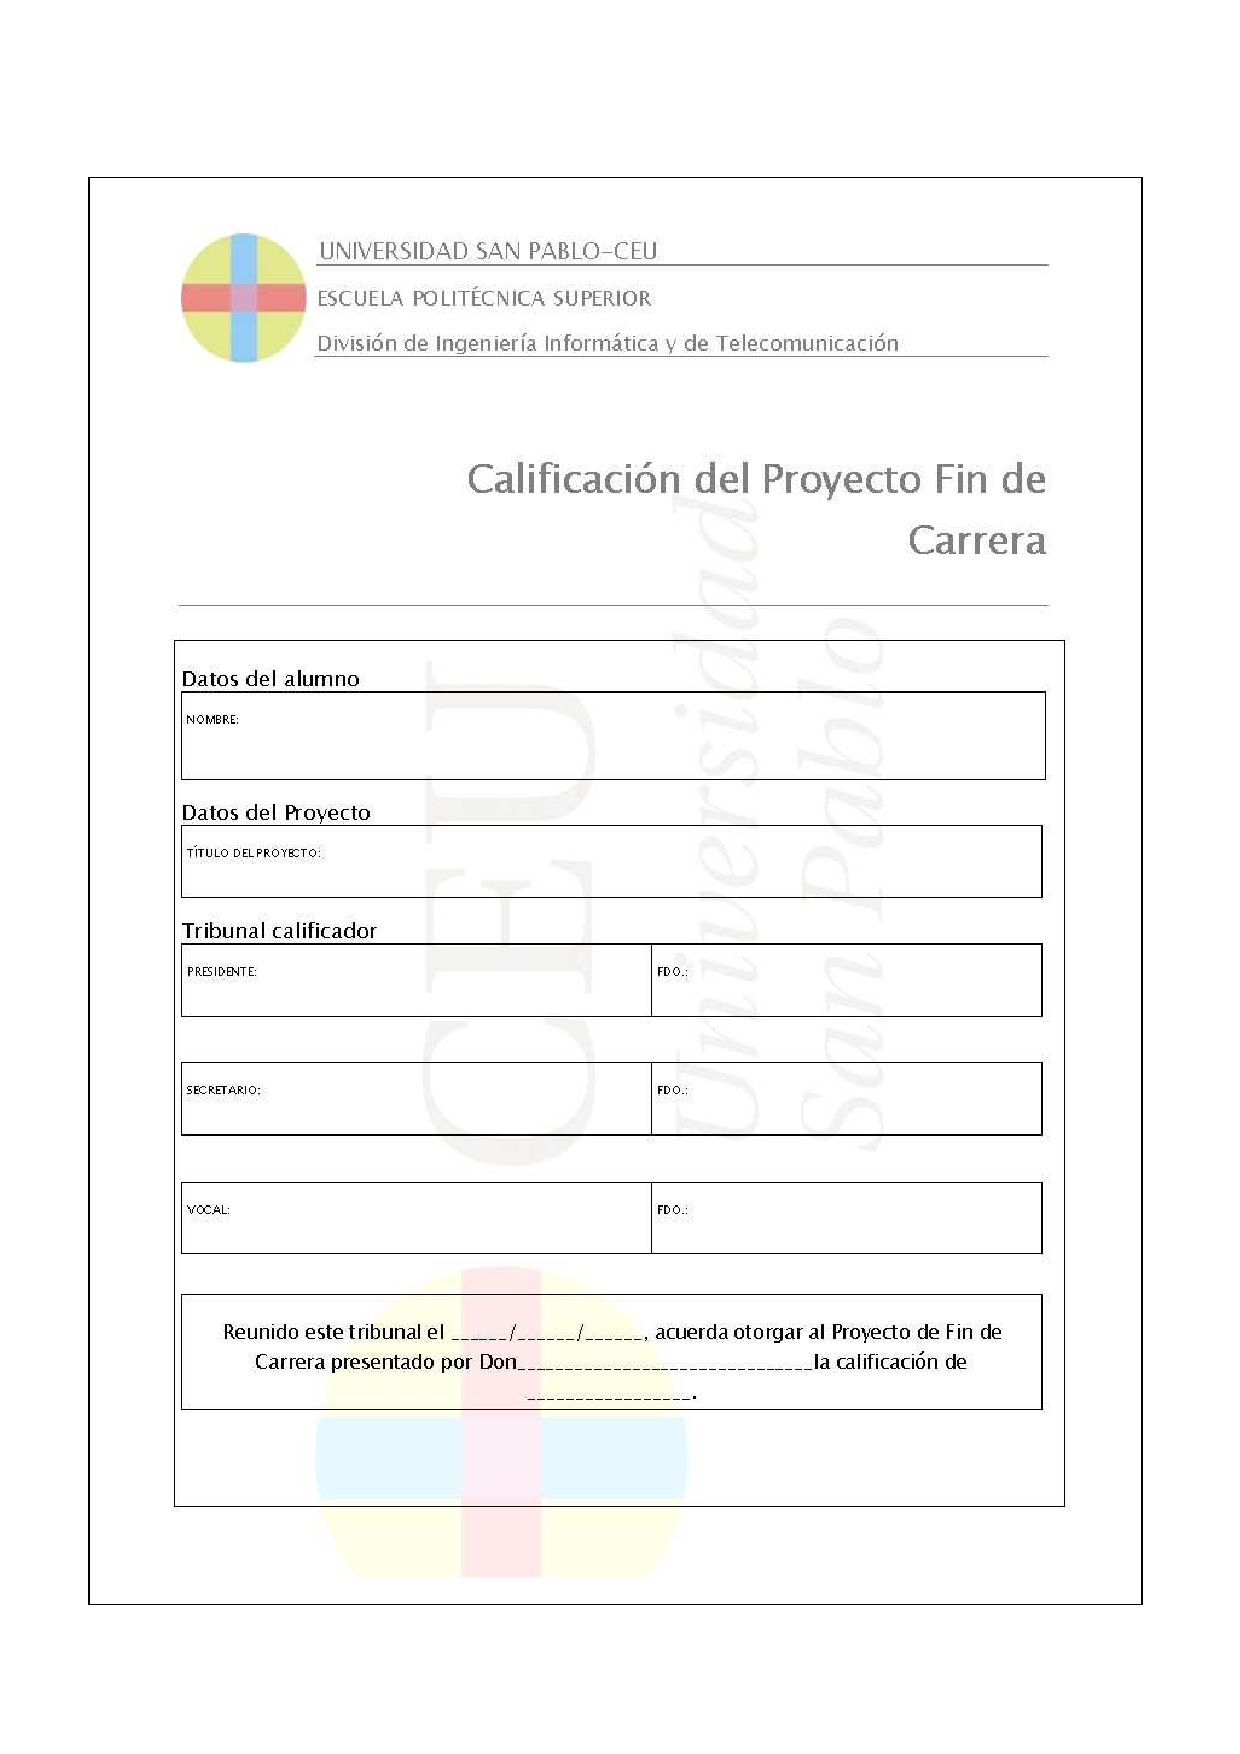
\includepdf[pages={1}]{pdf/calificacion.pdf}

%%%%%%%%%%%%%%%%%%%%%%%%%%%%%%%%%%%%%%%%%%%%%%%%%%%%%%%%%%%%%%%
% Dedicación
%%%%%%%%%%%%%%%%%%%%%%%%%%%%%%%%%%%%%%%%%%%%%%%%%%%%%%%%%%%%%%%
\begin{dedication}
Dedicated to my parents and sister \\
for their love, endless support \\
and encouragement.
\end{dedication}

%%%%%%%%%%%%%%%%%%%%%%%%%%%%%%%%%%%%%%%%%%%%%%%%%%%%%%%%%%%%%%%
% Abstracto
%%%%%%%%%%%%%%%%%%%%%%%%%%%%%%%%%%%%%%%%%%%%%%%%%%%%%%%%%%%%%%%

% Abstracto en español
\chapter*{Resumen}

Compañías como LG han presentado en los últimos años frigoríficos inteligentes; frigoríficos que se pueden controlar a través del móvil y permiten conocer los productos que hay en su interior a través de etiquetas inteligentes. 

El objetivo del proyecto es traer parte de esta tecnología al sin tener que realizar una gran inversión. No será necesario cambiar de frigorífico, para ello se ha creado un componente gracias a \emph{Arduino} que nos permitirá leer los productos que introduzcamos o consumamos del frigorifico.

Existen aplicaciones que nos permiten llevar el gasto en el hogar, pero a diferencia de este proyecto, están pensadas para insertar un ticket de compra. Este proyecto permite escanear producto por producto, y gracias a una base de datos colaborativa, obtener el gasto total de la compra; distinguir por tipo de alimento... También podremos consultar nuestros hábitos de comidas, consultar que productos nos faltan y generar una lista de la compra, etc. 

Esta solución se divide en tres bloques principales:

 \begin{description}
    \item Componente electrónico

    Es la parte del proyecto más física donde se ha creado un aparato que permite la lectura de productos.

    Para ello se cuenta con dos modos de entrada de productos; a través del código de barras ó un lector RFID, y de una salida Wireless para comunicar al servidor la entrada de los productos.

    \item Servidor centralizado

    Es la parte lógica del proyecto, el encargado de recibir la información del componente electrónico, almacenarla y operar con ella para ofrecer a las aplicaciones cliente acceso a toda la información.

    \item Aplicación cliente

    Es la parte de comunicación donde toda la información es consumida por el usuario a través de gráficas, resúmenes, listados, etc.

    Mediante el cruce de datos generado por el componente electrónico y toda la información contenida en el servidor se le mostrará al cliente la siguiente información:
        \begin{itemize}
        \item Stock actual del frigorífico
        \item Estadísticas de consumo; listados y estadísticas con los productos que se han comprado mediante el uso de filtros como; tipo de productos, fechas, precios...
        \item Estadísticas de gastos
        \end{itemize}

    Al emplear un servidor centralizado se va a permitir la creación de herramientas de colaboración entre los usuarios de la aplicación para la administración y creación de:
        \begin{itemize}
        \item Identificación de productos; nombre, precio, imagen, etc.
        \item Planes de compra; permitirá compartir planes de compra que pueden orientarse a distintos fines como el conseguir un ahorro económico.
        \item Recetas; de esta manera se podrá consultar en base al stock que se dispone en el frigorífico que recetas de cocina se pueden preparar.
        \end{itemize}
\end{description}

% Abstracto en inglés
\chapter*{Abstract}
This is the abstract

%%%%%%%%%%%%%%%%%%%%%%%%%%%%%%%%%%%%%%%%%%%%%%%%%%%%%%%%%%%%%%%
% Índice autogenerado
%%%%%%%%%%%%%%%%%%%%%%%%%%%%%%%%%%%%%%%%%%%%%%%%%%%%%%%%%%%%%%%

\tableofcontents

%%%%%%%%%%%%%%%%%%%%%%%%%%%%%%%%%%%%%%%%%%%%%%%%%%%%%%%%%%%%%%%
% Capítulos
%%%%%%%%%%%%%%%%%%%%%%%%%%%%%%%%%%%%%%%%%%%%%%%%%%%%%%%%%%%%%%%

\input{introduccion/fribone-introduccion}

\chapter{ESTADO DE LA CUESTIÓN}

En este capítulo se va a hacer un estudio de la tecnología existente para llevar las cosas a Internet en el hogar. En concreto se profundizará en Domótica para casas inteligentes y en los distintos componentes que nos permiten desarrollar nuevos conceptos de forma sencilla.

\section{DOMÓTICA}

El término domótica proviene de la unión de las palabras \emph{domus} (que significa casa en latín) y \emph{tica} (de automática, palabra en griego). La Real Academa Española lo define como el <<conjunto de sistemas que automatizan las diferentes instalaciones de una vivienda>>.

En este proyecto se utilizará el concepto de domótica como la tecnología aplicada al Internet de las Cosas en el hogar, es decir, conectar nuestro hogar a la nube.

\subsection{Historia}

\parpic[r][]{
    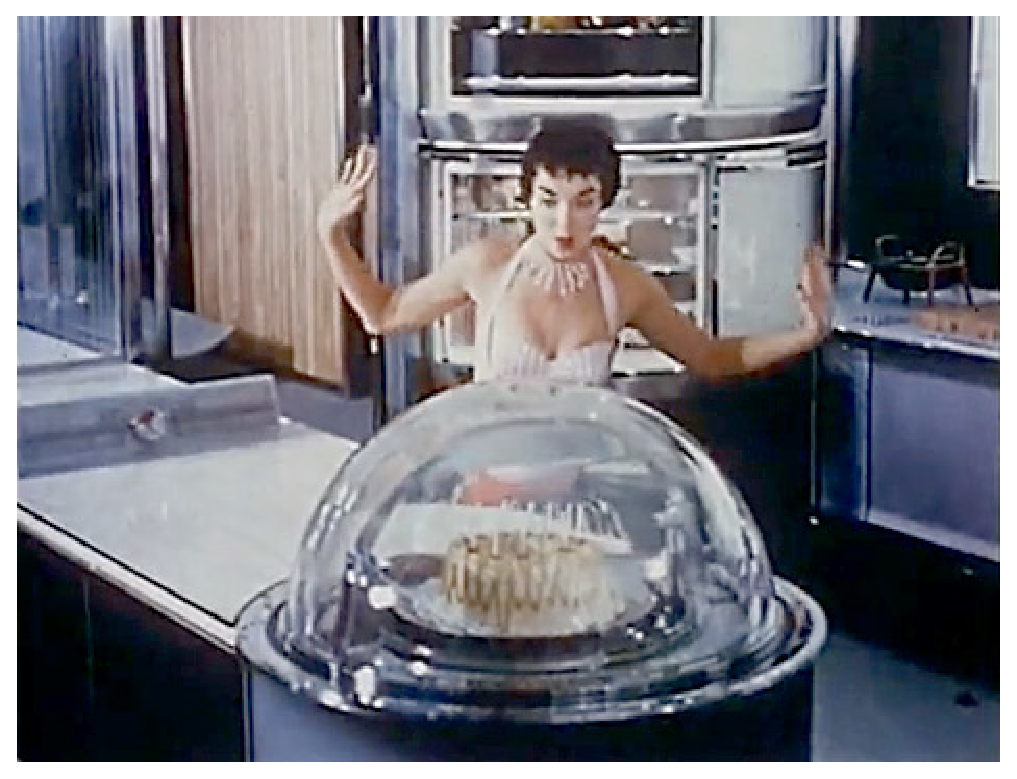
\includegraphics[keepaspectratio,width=0.25\textwidth]{Design_for_Dreaming_-_Cake_Under_Glass.eps}
    \label{fig:design-for-dreaming}
}

El hogar inteligente y automático comenzó a imaginarse en historias de ciencia ficción a inicios del siglo XX. En 1956 se emitió la película \emph{Design for Dreaming}~\ref{fig:design-for-dreaming} donde una mujer cae dormida y tiene una serie de sueños futuristas, incluyendo a \emph{Frigidaire}, la cocina automatizada del futuro. De ahí que no se pueda establecer una fecha concreta donde establecer el inicio de la domótica.

No obstante, si hemos de establecer una fecha de importante tenemos que hablar de 1975 con la aparición de \emph{X10}, un protocolo de comunicación que básicamente permite el control de las luces del hogar, para ello, utiliza la línea eléctrica como medio de comunicación. Debido a las limitaciones del protocolo de comunicación\emph{X10} se han desarrollado nuevas tecnologías para suplir estas carencias; CEBus, EIB, KNX...

A continuación se va a dar una breve explicación de cada una de estas tecnologías existentes en el mercado.

\subsection{X10}

\emph{X10} es un protocolo de comunicación para el control remoto de dispositivos eléctricos. Fue desarrollado en 1978 por \emph{Pico Electronics of Glenrothes}, Escocia, siendo la primera tecnología domótica en aparecer.

\parpic[r][]{
    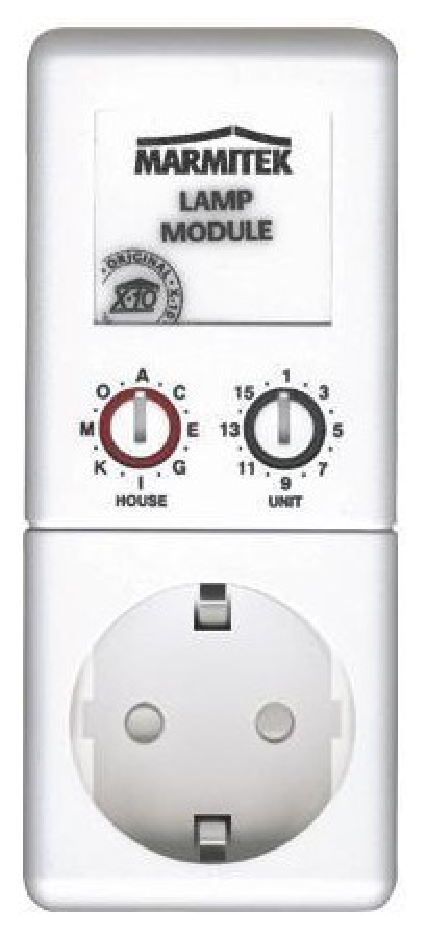
\includegraphics[keepaspectratio,width=0.09\textwidth]{modulo-lampara-x10.eps}
    \label{fig:modulo-lampara-x10}
}

Utiliza el cableado eléctrico como medio de comunicación que, debido a la limitación en ancho de banda que proporciona, solo es capaz de soportar hasta 256 dispositivos. A pesar de ello, es una tecnología ampliamente utilizada en Norteamérica y Europa por su característica de autoinstalable, sin necesidad de cableado adicional.

Las señales de control de X10 se basan en la transmisión de ráfagas de pulsos de \emph{RF} (120 kHz) que representan información digital. Estos pulsos se sincronizan en el cruce por cero de la señal de red (50 Hz ó 60 Hz). Con la presencia de un pulso en un semiciclo y la ausencia del mismo en el semiciclo siguiente se representa un '1' lógico y a la inversa se representa un '0'. A su vez, cada orden se transmite 2 veces, con lo cual toda la información transmitida tiene cuádruple redundancia. Cada orden involucra 11 ciclos de red (220 ms para 50 Hz y 183,33, para 60Hz).

Primero se transmite una orden con el Código de Casa y el Número de Módulo que direccionan el módulo en cuestión. Luego se transmite otro orden con el código de función a realizar (Function Code).

A continuación se muestra la tabla con los códigos que soporta el protocolo:

\begin{table}[!hbt]
    \begin{center}
        \begin{tabular}{|l |l | c | c |}
            \hline
            Código & Función & Unidireccional & Bidireccional \\
            \hline
            0 0 0 0 & All units off & X &  \\
            \hline
            0 0 0 1 & All lights on & X &  \\
            \hline
            0 1 1 0 & All lights off & X &  \\
            \hline
            0 0 1 0 & On & X &  \\
            \hline
            0 0 1 1 & Off & X &  \\
            \hline
            0 1 0 0 & Dim & X &  \\
            \hline
            0 1 0 1 & Bright & X &  \\
            \hline
            0 1 1 1 & Extended code & & X \\
            \hline
            1 0 0 0 & Hail request & & X \\
            \hline
            1 0 0 1 & Hail acknowledge & & X \\
            \hline
            1 0 1 0 & Pre-set dim & & X \\
            \hline
            1 1 0 1 & Status is on & & X \\
            \hline
            1 1 1 0 & Status is off & & X \\
            \hline
            1 1 1 1 & Status request & & X \\
            \hline
        \end{tabular}
        \caption{Listado de comandos \emph{X10}}
    \end{center}
\end{table}

\subsection{CEBus}

Bajo la necesidad de mejorar la limitada capacidad del protocolo \emph{X10} surgió \emph{CEBus}. El estándar \emph{CEBus} se desarrolló por la EIA (Electronic Industries Allianza) y su primera especificación salió en 1992.

\emph{CEBus}, a diferencia de \emph{X10}, se comunica sobre varias tecnologías; cableado eléctrico; cable coaxial; infrarrojos; radio frecuencia y cable óptico.

\subsection{EIB}

EIB

\subsection{KNX}

KNX

\section{ARDUINO}

Una buena definición de lo que es Arduino lo da la Wikipedia; <<Arduino es una plataforma de hardware libre, basada en una placa con un microcontrolador y un entorno de desarrollo, diseñada para facilitar el uso de la electrónica en proyectos multidisciplinares.>>.

Para este proyecto de fin de grado se va a utilizar \emph{Arduino} para desarrollar el hardware que permita la lectura de códigos de barras de los productos. Para ello se va a contar con una placa \emph{Arduino Yún} y distintos componentes como una pantalla TFT, un lector de código de barras, resistencias, pulsadores, etc.

A continuación se va a explicar brevemente el hardware \emph{Arduino}, \emph{Arduino Yún}, una pantalla TFT desarrollada para \emph{Arduino}, un lector RFID y un lector de código de barras.

\subsection{Hardware}

El hardware consiste en una placa con un microcontrolador \emph{Atmel AVR} y puertos de entrada/salida. Los microcontroladores más usados son el \emph{Atmega168}, \emph{Atmega328}, \emph{Atmega1280}, \emph{ATmega8} por su sencillez y bajo coste que permiten el desarrollo de múltiples diseños.

\begin{figure}[h!]
    \centering
    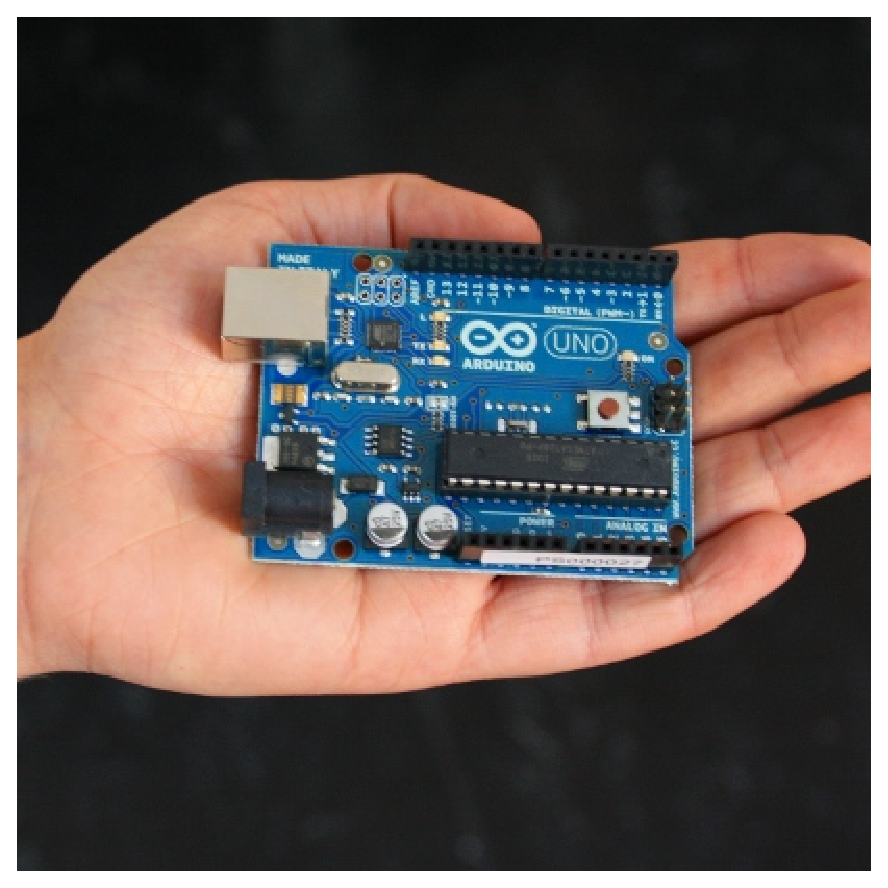
\includegraphics[keepaspectratio,width=0.6\textwidth]{arduino_uno_test.eps}
    \caption{Arduino uno}\label{fig:arduino_uno_test}
\end{figure}


Por otro lado el software consiste en un entorno de desarrollo que implementa el lenguaje de programación \emph{Wiring} y el cargador de arranque que es ejecutado en la placa.

\begin{figure}[h!]
    \centering
    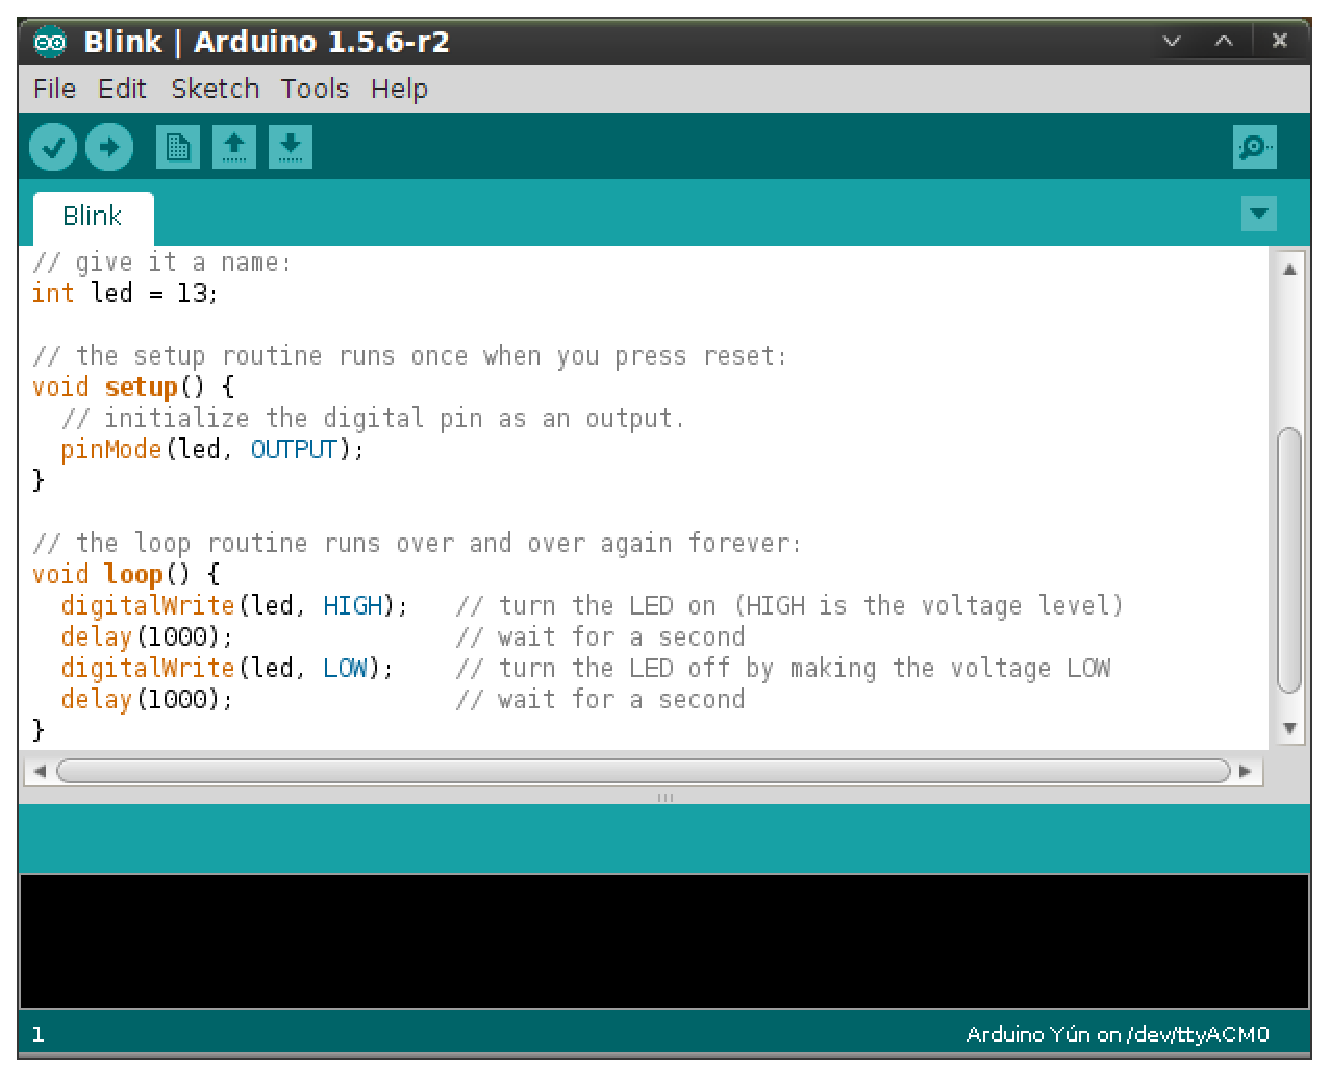
\includegraphics[keepaspectratio,width=0.6\textwidth]{arduino-ide.eps}
    \caption{IDE Arduino}\label{fig:arduino-ide}
\end{figure}

El lenguaje de alto nivel \emph{Wiring}, implementado en C/C++, permite una programación sencilla del hardware. Comparte todas las funciones estándar de C, algunas de C++ y añade las propias para el manejo de puertos (digitales, analógicos).

A continuación se muestra un código sencillo para hacer parpadear un diodo led cada segundo, se utiliza el puerto 8 digital de la placa \emph{Arduino}:

\begin{lstlisting}
    void setup() {
      pinMode(8, OUTPUT);
    }

    boolean encendido = false;
    void loop() {
      if(!encendido) {
        digitalWrite(8, HIGH);
      } else {
        digitalWrite(8, LOW);
      }
      encendido!=encendido;
      delay(1000);
    }
\end{lstlisting}

\subsection{Arduino Yún}

Existen una gran variedad de placas Arduino, tanto oficiales como no oficiales; Arduino uno, Arduino Mega, Arduino Leonardo... Y una de las más recientes, la cual usaré en este proyecto, es la placa \emph{Arduino Yún}.

\begin{figure}[h!]
    \centering
    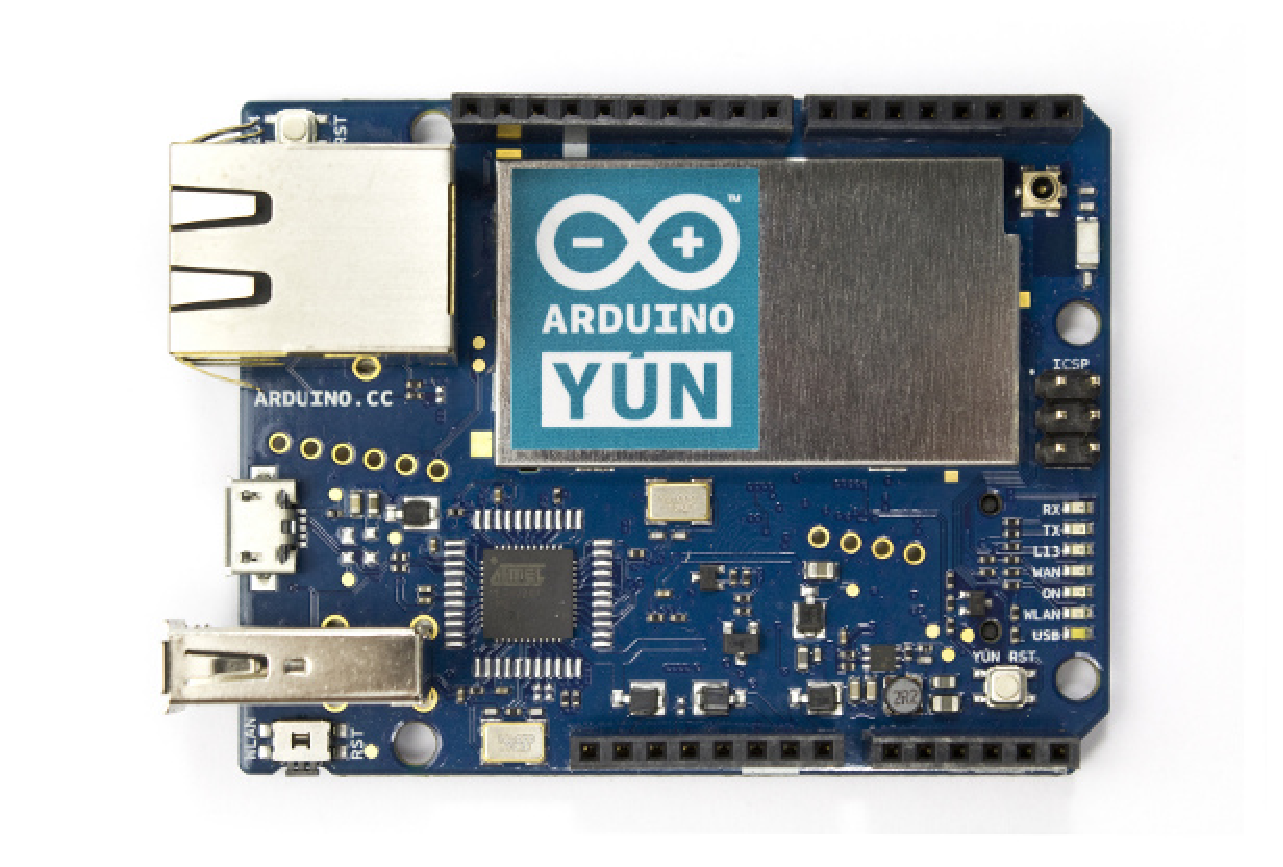
\includegraphics[keepaspectratio,width=0.6\textwidth]{arduino_yun_front.eps}
    \caption{Frontal arduino}\label{fig:arduino-yun-front}
\end{figure}

La ventaja principal, y por la que me he decantado por comprar esta placa, es la combinación de Arduino (\emph{microcontrolador ATmega 32U4}) con un sistema operativo Linux (\emph{microprocesador AR9331}) con conectividad WiFi. Esto permite utilizar todo el potencial de Arduino en el desarrollo de nuestro hardware y obtener todo el potencial de una máquina Linux, a través del sistema operativo \emph{Linino}, para ejecutar comandos, scripts, aplicaciones y cualquier cosa que se nos ocurra.

\begin{figure}[h!]
    \centering
    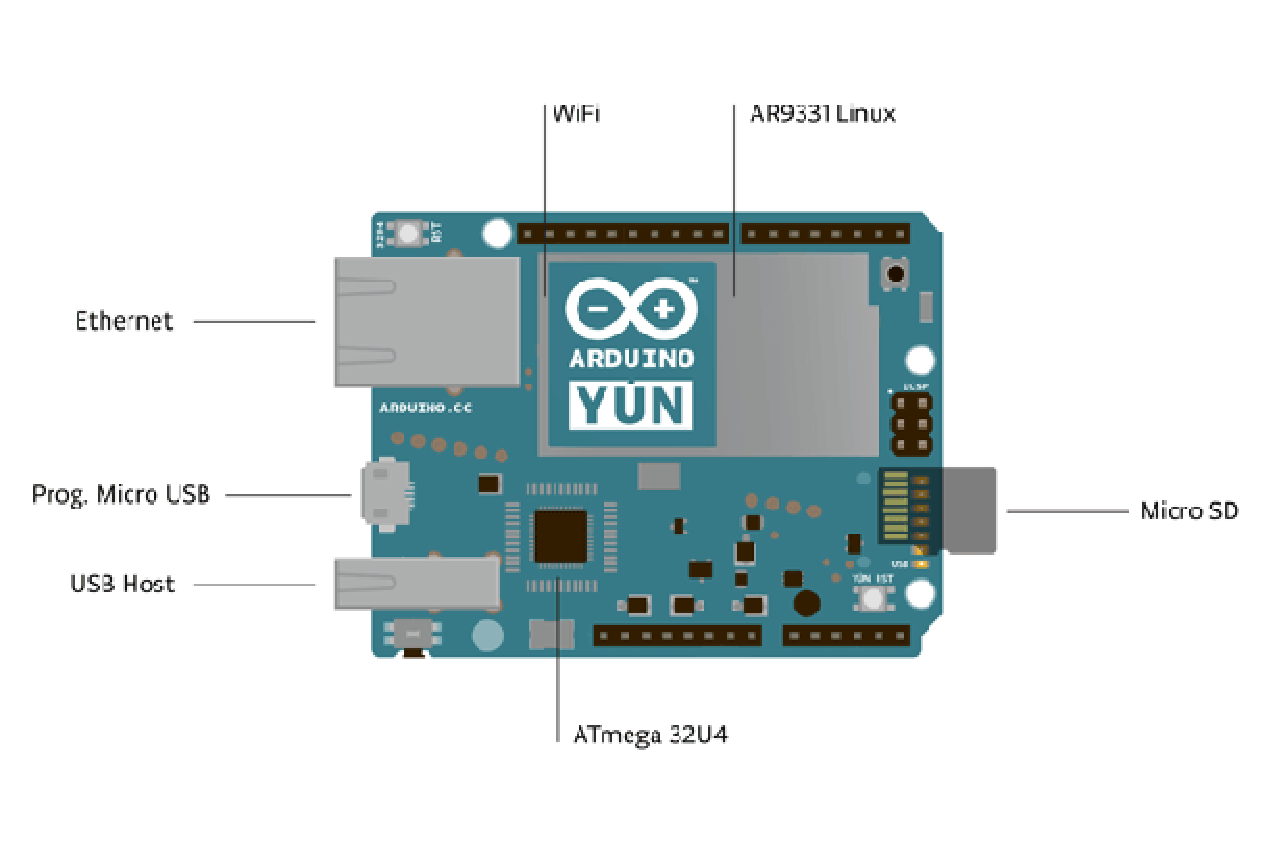
\includegraphics[keepaspectratio,width=0.6\textwidth]{arduino_parts.eps}
    \caption{Componentes de arduino}\label{fig:arduino-parts}
\end{figure}

La comunicación entre Arduino y Linux se realiza a través de la librería \emph{Bridge}, facilitando el intercambio de información y órdenes entre ambos micros. La librería da el potencial al microcontrolador de ejecutar scripts, comunicarse con interfaces de red, tener acceso a una memoria compartida entre el microprocesador y el microcontrolador, acceder al sistema de ficheros...

Las características de \emph{Arduino Yún} son las siguientes:

\textbf{AVR Arduino microcontroller}

\begin{tabular}{| l | l |}
\hline
Microcontroller & ATmega32u4 \\ \hline
Operating Voltage & 5V \\ \hline
Input Voltage & 5V \\ \hline
Digital I/O Pins & 20 \\ \hline
PWM Channels & 7 \\ \hline
Analog Input Channels & 12 \\ \hline
DC Current per I/O Pin & 40 mA \\ \hline
DC Current for 3.3V Pin & 50 mA \\ \hline
Flash Memory & 32 KB (of which 4 KB used by bootloader) \\ \hline
SRAM & 2.5 KB \\ \hline
EEPROM & 1 KB \\ \hline
Clock Speed & 16 MHz \\ \hline
\end{tabular}

\textbf{Linux microprocessor}

\begin{tabular}{| l | l |}
\hline
Processor & Atheros AR9331 \\ \hline
Architecture & MIPS @400MHz \\ \hline
Operating Voltage & 3.3V \\ \hline
Ethernet & IEEE 802.3 10/100Mbit/s \\ \hline
WiFi & IEEE 802.11b/g/n \\ \hline
USB Type-A & 2.0 Host/Device \\ \hline
Card Reader & Micro-SD only \\ \hline
RAM & 64 MB DDR2 \\ \hline
Flash Memory & 16 MB \\ \hline
\end{tabular}


\subsection{Pantalla TFT}

Uno de los componentes para dotar de comunicación a nuestra placa Arduino es utilizar una pantalla TFT. Existen variedad de pantallas TFT; diferentes dimensiones, con soporte táctil, mayor rapidez de refresco... Para el proyecto he optado por comprar la oficial de Arduino:

\begin{figure}[h!]
    \centering
    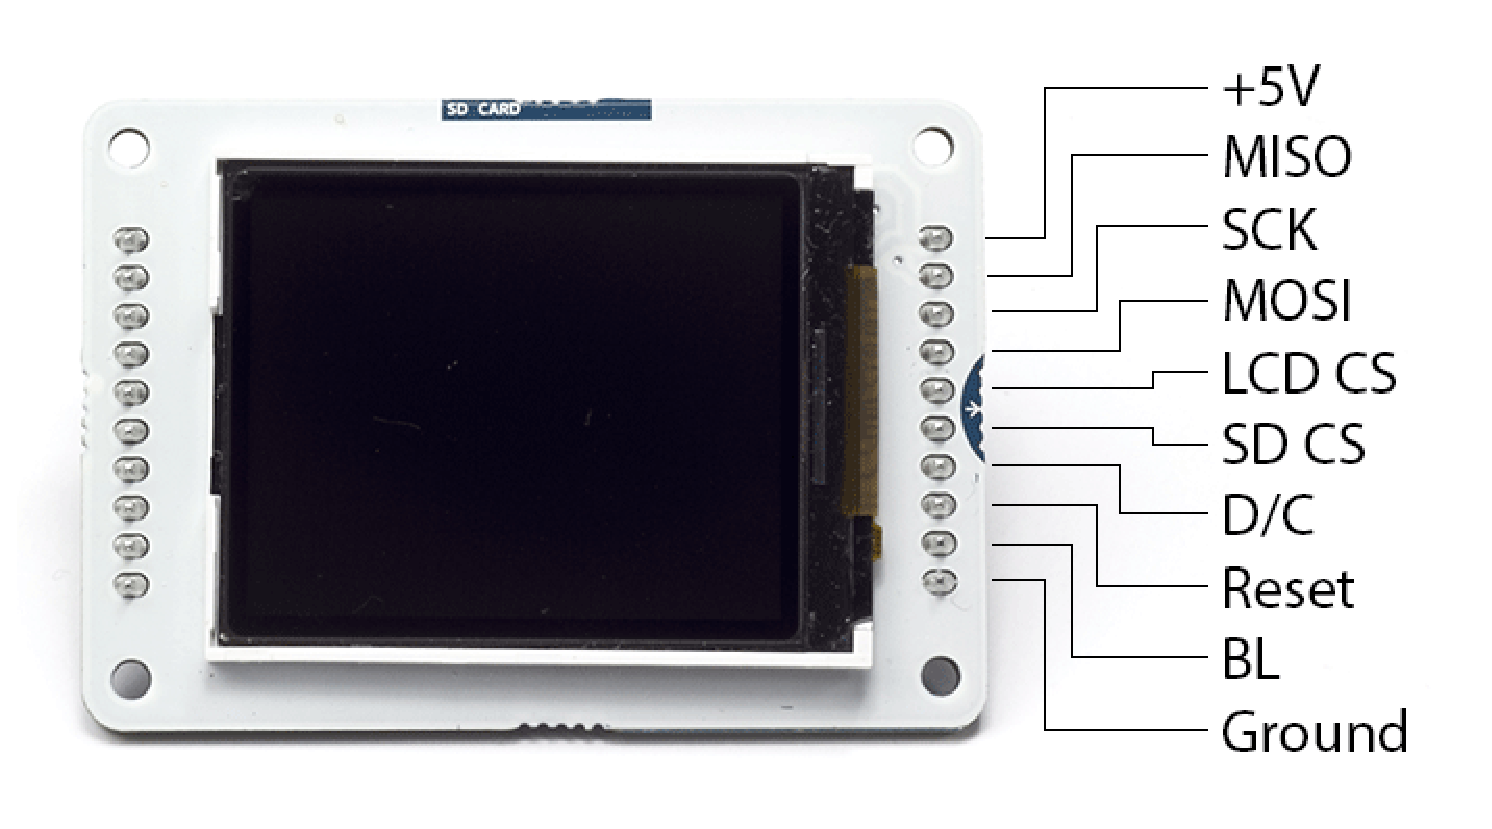
\includegraphics[keepaspectratio,width=0.6\textwidth]{pantalla_tft_front.eps}
    \caption{Pantalla TFT}\label{fig:arduino-tft-front}
\end{figure}


\parpic[r][]{
    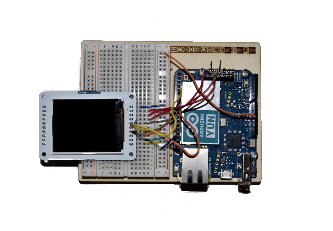
\includegraphics[keepaspectratio,width=0.38\textwidth]{arduino_conexiones.eps}
    \label{fig:arduino_conexiones}
}

Es una pantalla de 1,77" de diagonal, con 160x128 pixels de resolución, y con un lector de tarjetas microSD para cargar imágenes. La pantalla está pensada para encajar con las placas \emph{Arduino Esplora} ó \emph{Arduino Robot}, con el resto de placas Arduino se pueden realizar las conexiones a mano.

A través de la librería \emph{TFT} se pueden dibujar elementos en la pantalla o, mediante una memoria microSD, cargar imágenes en la pantalla. A continuación se expone una manera para dibujar un círculo y un cuadrado en la pantalla:

\begin{lstlisting}
    ...

    void setup() {
      TFTscreen.begin();
      TFTscreen.background(255, 255, 255);

    }

    void loop() {
      TFTscreen.stroke(0,0,0);
      TFTscreen.fill(127,127,127);
      TFTscreen.circle(TFTscreen.width()/2, TFTscreen.height()/2, 30);

      TFTscreen.fill(50,40,30);
      TFTscreen.rect(TFTscreen.width()/2, TFTscreen.height()/2, 30, 30);

      delay(1500);
    }
\end{lstlisting}

A continuación se muestra una captura de como se visualiza el dibujo en la pantalla:

\begin{figure}[h!]
    \centering
    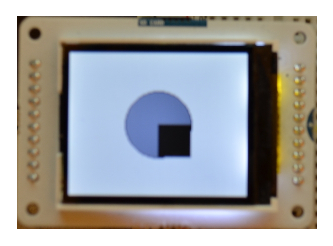
\includegraphics[keepaspectratio,width=0.4\textwidth]{tft_circulo_cuadrado.eps}
    \caption{TFT - Dibujando}\label{fig:tft_circulo_cuadrado}
\end{figure}

En cambio, para cargar una imagen desde la tarjeta de memoria y mostrarla en la pantalla TFT, primero se tiene queesperar a que la memoria SD esté inicializada y a continuación, leer la imagen y renderizarla en pantalla:

\begin{lstlisting}
    ...

    void setup() {
      TFTscreen.begin();
      TFTscreen.background(255, 255, 255);

      if (!SD.begin(sd_cs)) {
        return; // Error SD
      }
    }

    void loop() {
      logo = TFTscreen.loadImage("f1.bmp");
      TFTscreen.image(logo, 0, 0);
      delay(1500);
    }
\end{lstlisting}

A continuación se muestra una captura de como se visualiza la imagen en la pantalla:

\begin{figure}[h!]
    \centering
    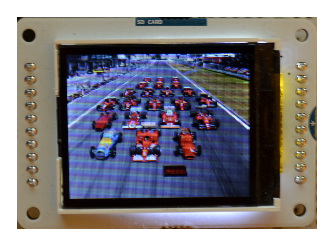
\includegraphics[keepaspectratio,width=0.4\textwidth]{tft_f1.eps}
    \caption{TFT - Imagen}\label{fig:tft_f1}
\end{figure}

\subsection{RFID}

\parpic[r][]{
    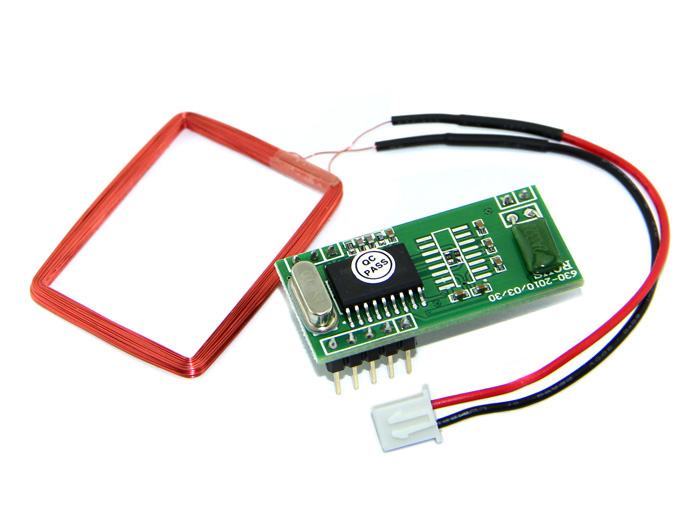
\includegraphics[keepaspectratio,width=0.38\textwidth]{lector_rfid.png}
    \label{fig:lector_rfid}
}

El lector \emph{RFID} es uno de los componentes empleados para poder escanear productos. En concreto se ha utilizado para el proyecto un lector \emph{RFID de 125K} con las siguientes características:

\begin{itemize}
    \item Working voltage: 3.5-5V
    \item Frequency: 125Khz
    \item Baud rate: 9600
    \item Interface Type: TTL Level RS232 format
    \item Reception range: 30mm~50mm
\end{itemize}

El código para trabajar con el lector \emph{RFID} es muy sencillo, la única ''complicación'' es tener que utilizar la librería \emph{SoftwareSerial} para simular dos pines como puerto serie (ya que \emph{Arduino Yún} tiene reservados los pines 0 y 1 de puerto serie para la comunicación con Linux a través de la librería bridge).

No se pueden utilizar los pines dedicados de puerto serie (\emph{0 y 1}) ya que \emph{Arduino Yún} los utiliza para la comunicación entre el microcontrolador \emph{ATmega32U4} y el microprocesador \emph{Atheros AR9331} a través de la librería \emph{Bridge}.

El código utilizado para escanear tarjetas \emph{RFID} es el siguiente:

\begin{lstlisting}
//Lector RFID
#include <SoftwareSerial.h>
#define rxPin 11
#define txPin 12
SoftwareSerial RFID = SoftwareSerial(rxPin, txPin); // RX and TX
char arrayTag[10];

void setup() {
    RFID.begin(9600);
}

void loop() {
    if(leerYProcesarEtiquetaRFID()) {
        // Hacer algo
    }
}

boolean leerYProcesarEtiquetaRFID() {
  int leidoTag = 0;

  String tag;
  while(RFID.available() > 0) {
      leidoTag = 1;
      int rfid = RFID.read();

      if(rfid != 13 && rfid != 10) {
         tag += (char)rfid;
      }
  }
  if(leidoTag) {
    tag.toCharArray(arrayTag, 10);
  }

  return leidoTag != 0;
}
\end{lstlisting}

\subsection{Lector de código de barras}

Además de utilizar como método de entrada un lector \emph{RFID} se ha utilizado otro método tradicional, el lector de código de barras. Para ello se ha buscado un lector que sea \emph{USB HID}, es decir, que no necesite la instalación de drivers para funcionar.

\begin{figure}[h!]
    \centering
    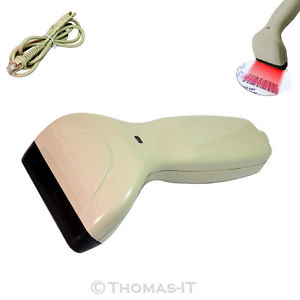
\includegraphics[keepaspectratio,width=0.4\textwidth]{lector_codigo_barras.png}
    \caption{Lector de código de barras}\label{fig:lector_codigo_barras}
\end{figure}

En la sección \emph{COMPONENTE HARDWARE} se explica la configuración de \emph{Arduino Yún} y como se decodifica la entrada de dígitos del lector con \emph{Python}.

\section{COMPARATIVA CON OTROS COMPONENTES}

La elección de \emph{Arduino Yún} se ha realizado teniendo en cuenta las alternativas existentes en el mercado, encontrando que es la más adecuada para el tipo de proyecto que se va a realizar. A continuación se muestran algunos de los componentes que se han tenido en cuenta.

\subsection{Raspberry PI}

\parpic[r][]{
    \includegraphics[keepaspectratio,width=0.35\textwidth]{raspberry-pi.eps}
    \label{fig:arduino-yun}
}

La \emph{Raspberry Pi} es un computador de bajo coste y del tamaño de una tarjeta de crédito, el cual se puede conectar a un monitor o aun ordenador, junto a un teclado y un ratón. Permite realizar todo lo que puede hacer un ordenador de sobremesa; navegar por internet, reproducir vídeo en alta definición, programas de ofimática e incluso correr videojuegos. Además, la placa de \emph{Raspberry Pi} cuenta con 8 pines GPIO que permiten controlar componentes electrónicos como leds, pulsadores, etc.

A diferencia de \emph{Arduino Yún} el propósito de la \emph{Raspberry PI} es ser ordenador en miniatura, corriendo un sistema Linux, y aunque pueda comunicarse a través de sus pines GPIO ese no es su propósito. \emph{Arduino Yún} en cambio es un microcontrolador especializado en controlar componentes, además de contar con la ventana de poseer un microprocesador con una versión de Linux. Para ello cuenta con un mayor número de pines entrada salida; analógicos, comunicación SPI... Que serán útiles para añadir componentes como un lector RFID, una pantalla TFT y botones para controlarla; así como se pueden añadir sensores de temperatura, distancia, etc. para poder controlar parámetros como la temperatura del frigorífico, la hora y el tiempo que ha estado abierto el frigorífico, etc.

\subsection{Z-Wave}

Z-Wave es el estándar internacional para la interconexión inalámbrica de los sistemas domóticos de su casa. Puede gestionar  la iluminación, la electricidad, las persianas, las alarmas, etc. Los productos Z-Wave de diferentes fabricantes trabajan bien juntos permitiendo el control completo de su hogar.

\begin{figure}[H]
    \centering
    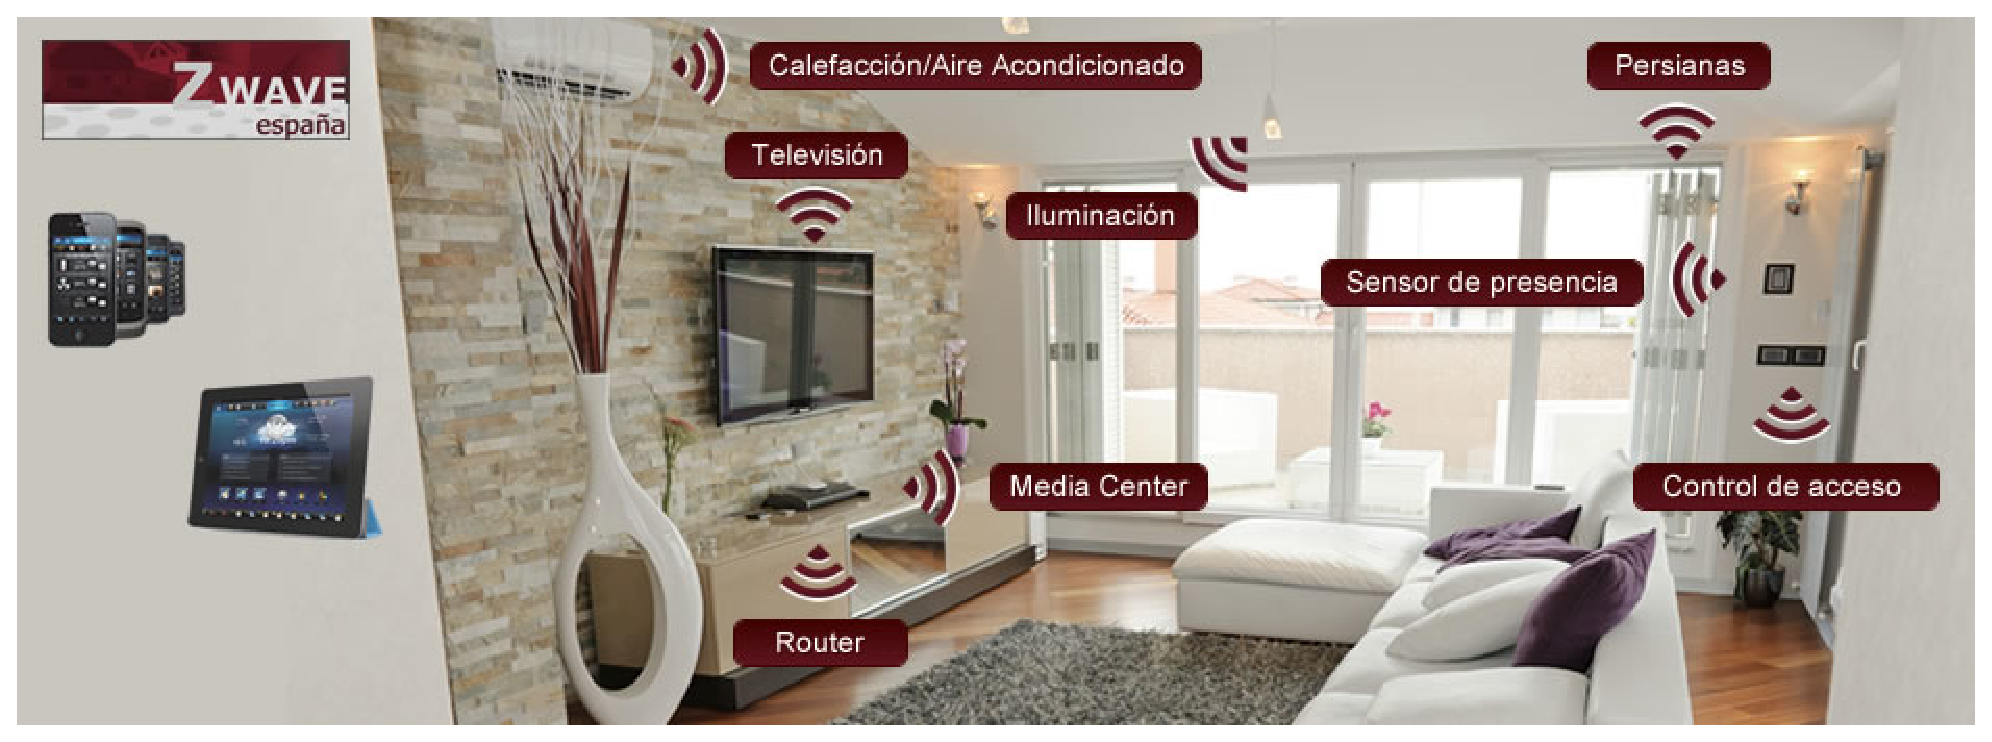
\includegraphics[keepaspectratio,width=0.9\textwidth]{z-wave.eps}
    \caption{Z-Wave}\label{fig:z-wave}
\end{figure}

La integración de \emph{Arduino} con el estándar \emph{Z-Wave} no es sencillo. Es posible encontrar módulos wireless que con compatibles con la frecuencia que emiten los componentes \emph{Z-Wave} pero hay que implementarse todo el protocolo \emph{Z-Wave} de comunicación, lo cual no es sencillo.

Además, si se optara por realizar esta integración, sería necesario contar un servidor \emph{Z-Wave} para realizar la comunicación. Y los productos de \emph{Z-Wave} tienen un precio bastante elevado, por lo que el coste final del proyecto ascendería, lo cual no cumple con uno de los objetivos de realizar un componente barato.

\section{CONCLUSIONES}

En resumen al estado de la cuestión se puede observar que a lo largo de la historia se han desarrollado múltiples tecnologías para facilitar y mejorar las condiciones de vida en el hogar a través de tecnología.

\parpic[r][]{
    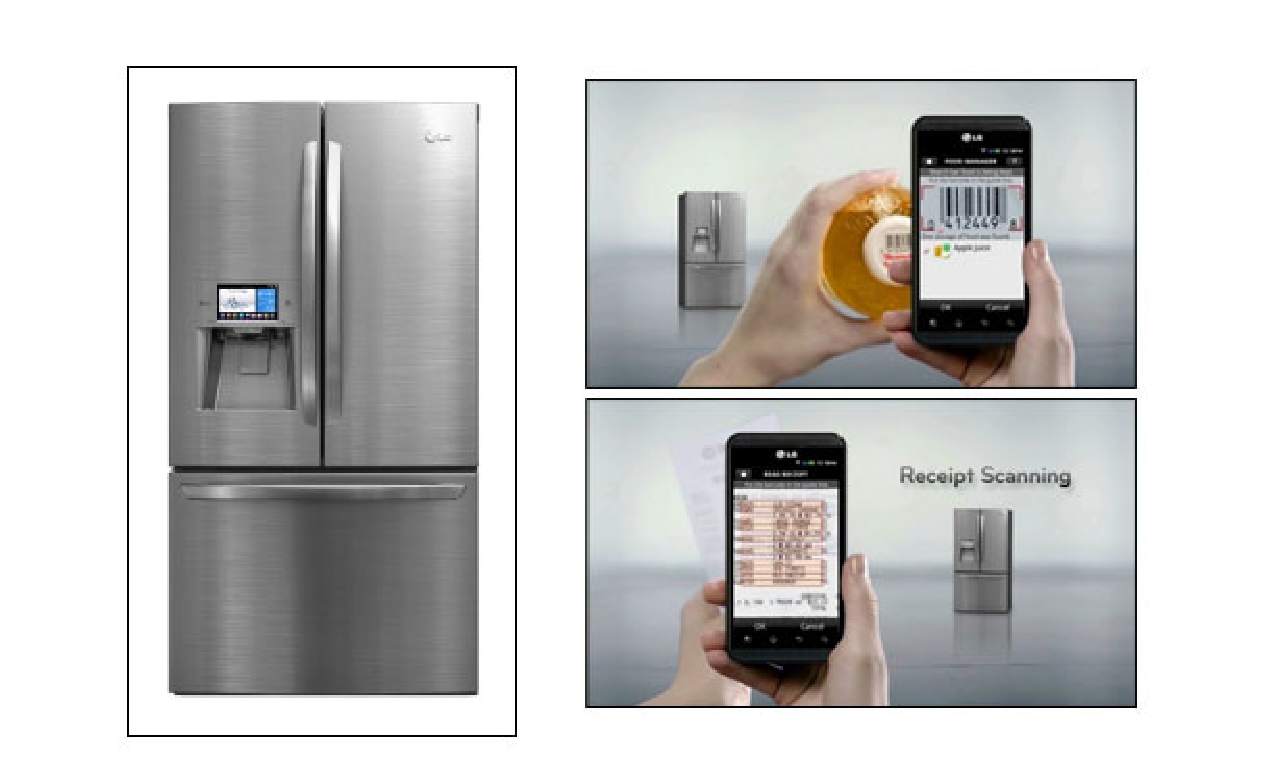
\includegraphics[keepaspectratio,width=0.38\textwidth]{frigo-lg.eps}
    \label{fig:frigo-lg}
}

A día de hoy existen proyectos para dotar de inteligencia a los frigoríficos, sin embargo, solamente son prototipos debido a su alto coste de fabricación.

Para traer al hogar parte de esta tecnología se ha aprovechado de los avances en hardware libre (a través de Arduino) para desarrollar un prototipo de frigorífico inteligente. Este protipo tendrá como objetivo dotar de inteligencia al frigorífico sin tener que realizar una gran inversión en hardware.

\chapter{REQUISITOS DEL SISTEMA}

\section{Introducción}

Esta especificación se ha elaborado inspirándose en las directrices dadas en la norma ANSI/IEEE 830-1998 [IEEE, 98].

\section{Propósito de este capítulo}

El objeto de la especificación es definir de manera clara y precisa todas las funciones y restricciones del sistema que se desea construir.

\section{Ámbito del sistema}

El objetivo de este proyecto es el de elaborar un sistema que permita dotar de inteligencia al frigorífico del hogar utilizando para ello una placa Arduino. El sistema deberá ser capaz de leer productos y transmitirlos a un servidor vía WiFi. El usuario entonces podrá consultar los productos que contiene su frigorífico a través de una aplicación.

\chapter{ARQUITECTURA DEL SISTEMA}

\section{Diagrama general}

Siguiendo los requisitos anteriormente explicados, se desarrolla un sistema basado en tres partes: componente hardware, servidor y aplicación cliente.

El diagrama general del sistema es el que se muestra en la siguiente figura:

\begin{figure}[H]
    \centering
    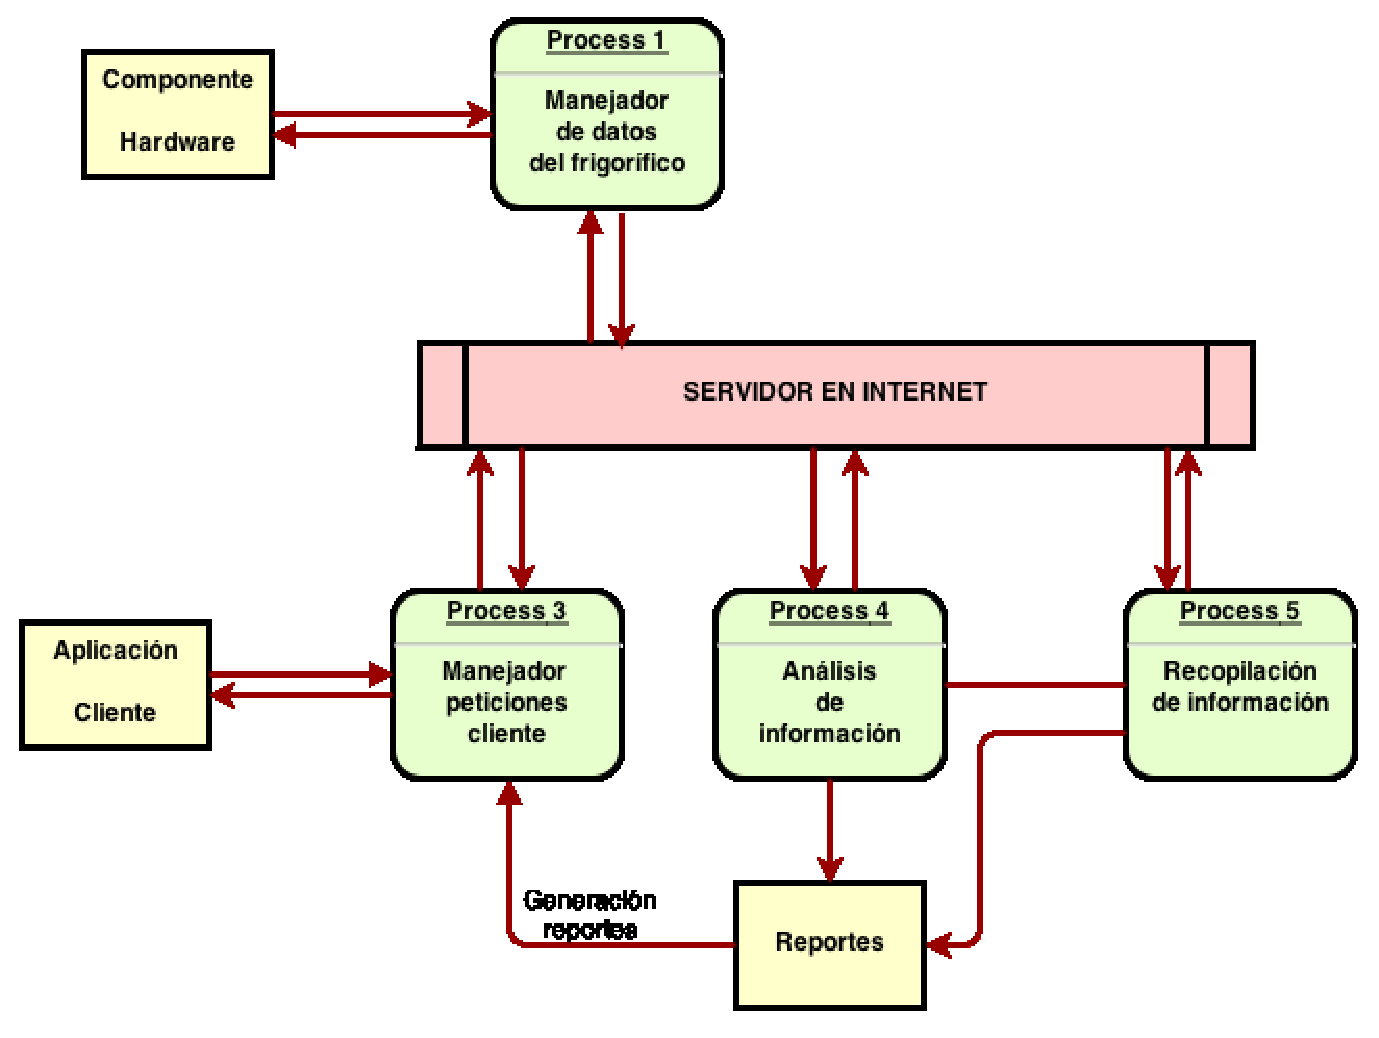
\includegraphics[keepaspectratio,width=0.9\textwidth]{diagrama-general.eps}
    \label{fig:diagrama-general}
\end{figure}

\section{Componente hardware}

Sección componente hardware

\section{Componente servidor}

El servidor es la pieza central de toda la arquitectura del proyecto, es el nexo común entre todas las interfaces del proyecto.

La comunicación entre las distintas interfaces se realiza a través de una API \emph{RESTful} que se caracteriza por:

\begin{itemize}
    \item Está basada en URIs, por ej: \url{http://example.com/resources}.
    \item Tipos de datos de Internet como \emph{JSON}.
    \item Métodos estándar HTTP: \emph{GET}, \emph{POST}, \emph{PUT} ó \emph{DELETE}.
    \item Uso de hipermedios
\end{itemize}

El lenguaje utilizado para el desarrollo del servidor es \emph{PHP} debido a que en prácticamente la totalidad de los servidores de viene por defecto. Mientras que el empleo de otros lenguajes de servidor, obligaría a contratar un servidor dedicado para poder realizar la instalación del mismo, aumentando los costes y la complejidad del proyecto.

\section{Componente cliente}

Dentro de toda la arquitectura del proyecto esta es la parte que cobra más importancia de cara al usuario. Se encarga de procesar toda la información contenida por el servidor y de presentarla en un formato amigable.

La comunicación con el servidor se realizará a través de la \emph{API RESTful} que se ha desarrollado. Gracias a esta API se pueden realizar aplicaciones cliente para distintas plataformas de manera sencilla.

Se ha desarrollado una aplicación cliente \emph{web}, utilizando para ello la api \emph{RESTful} proporcionada por el servidor, un sistema de plantillas basadas en \emph{handlebars} para renderizar las diferentes pantallas de presentación al cliente y \emph{JavaScript} para la programación desde el lado del cliente.

\chapter{DISEÑO E IMPLEMENTACIÓN}

Para la implementación del sistema se han utilizado diferentes lenguajes de programación y tecnologías que se irán comentando y describiendo a lo largo del capítulo.

\section{COMPONENTE HARDWARE}

El componente hardware se ha implementado utilizando dos lenguajes de programación; \emph{Wiring} para el microprocesador ATmega32u4, Python para el procesador \emph{Atheros AR9331}.

\subsection{Configurando el sistema}

El primer paso es configurar la placa de Arduino Yún para empezar a trabajar sobre ella. Para ello Yún corre una distribución de Linux llamada \emph{OpenWrt-Yun}, basado en \emph{OpenWrt}, la cual nos permite acceder vía \emph{ssh} o vía web para poder configurarla.

La primera vez que se conecta Arduino Yún se crea una red sin encriptar para poder conectarnos a ella y poder configurarla, el nombre de la red tiene el formato \emph{ArduinoYun-XXXXXXXXXXXX}. Una vez conectados se accede al panel web de configuración a través de la url \emph{http://arduino.local} y se nos muestra la siguiente ventana:

\begin{figure}[H]
    \centering
    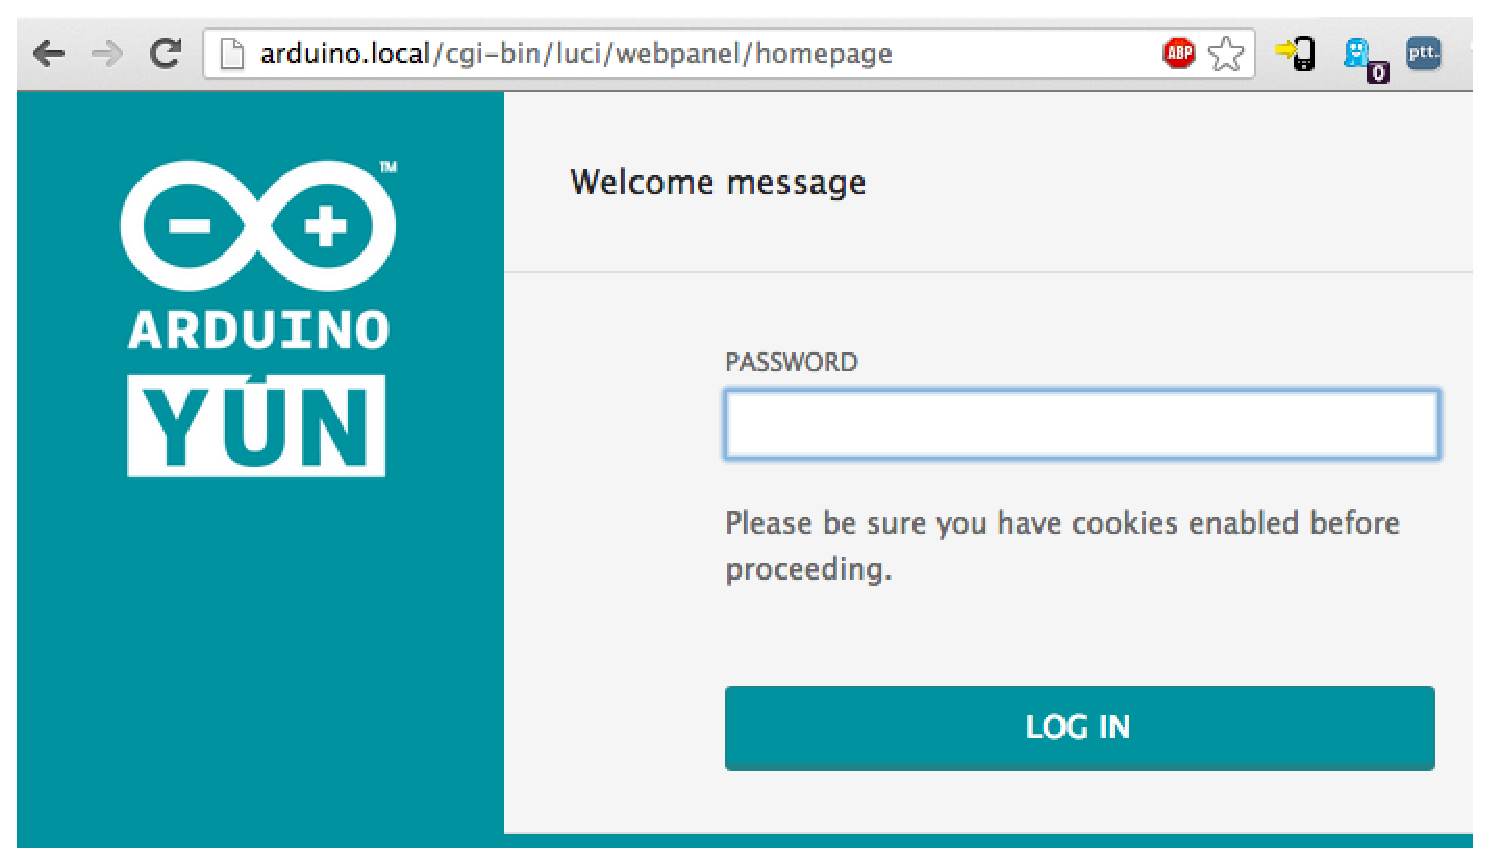
\includegraphics[keepaspectratio,width=0.6\textwidth]{YunWebPassword.eps}
    \caption{Arduino Yún Web Password}\label{fig:yun-web-password}
\end{figure}

La contraseña por defecto es \emph{Arduino} y nos permite acceder al panel de diagnóstico donde nos muestra información sobre la red WiFi y la conexión Ethernet. Además, nos permite acceder al panel de configuración:

\begin{figure}[H]
    \centering
    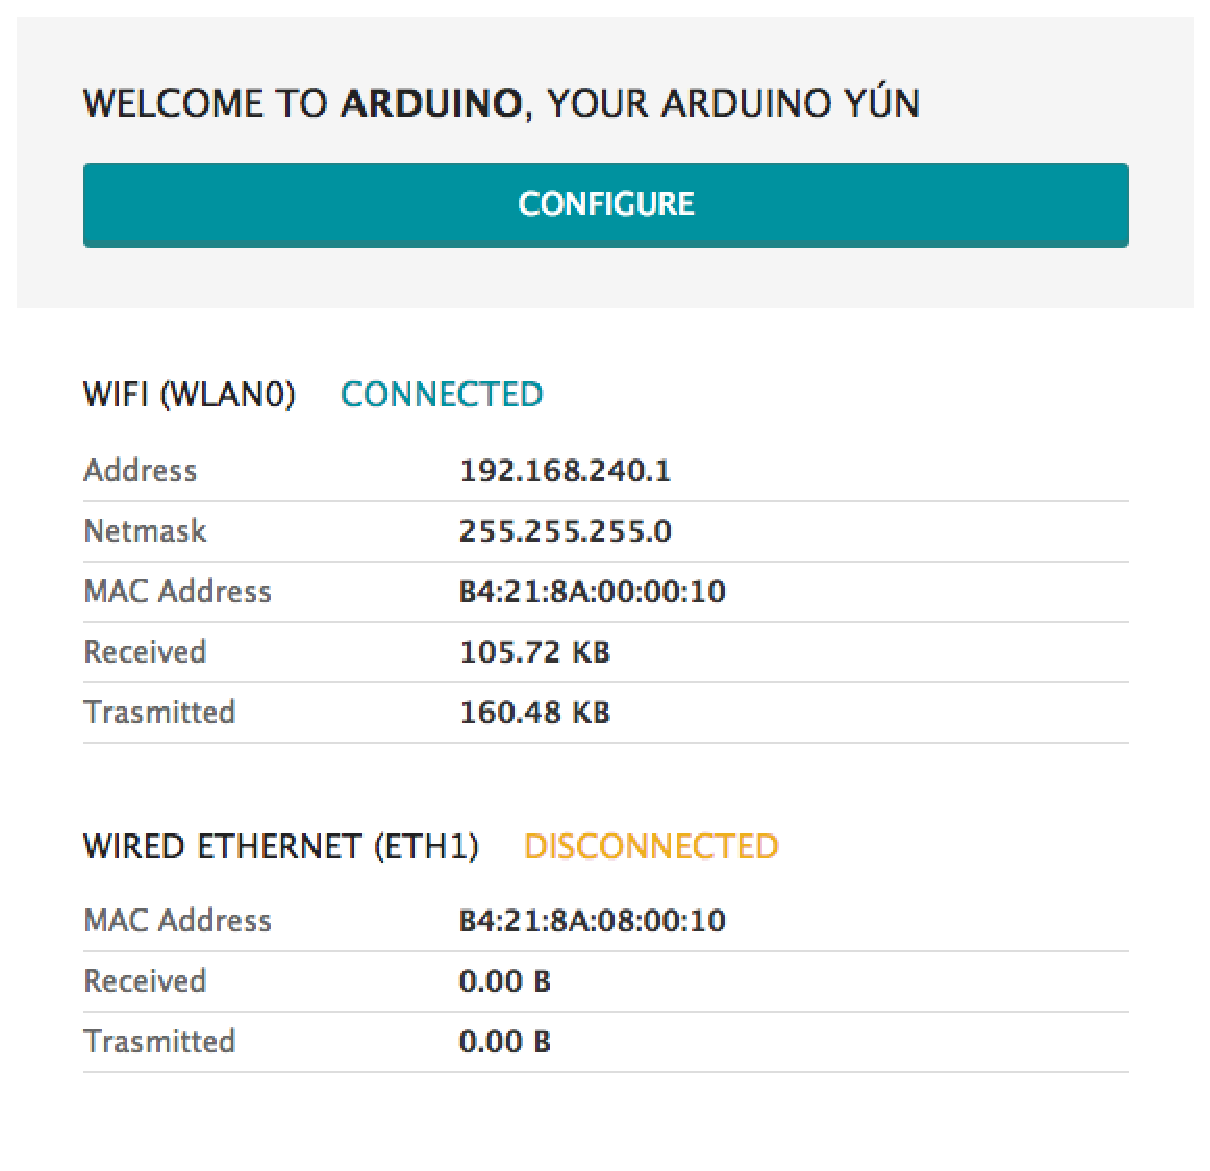
\includegraphics[keepaspectratio,width=0.6\textwidth]{YunWebDiagnostic.eps}
    \caption{Arduino Yún Web Diagnostic}\label{fig:yun-web-diagnostic}
\end{figure}

El panel de configuración nos permite nombrar nuestra placa Arduino, establecer una contraseña de acceso, configurar la zona horaria y por último, y lo más importante, decirle a que red WiFi debe conectarse.

\begin{figure}[H]
    \centering
    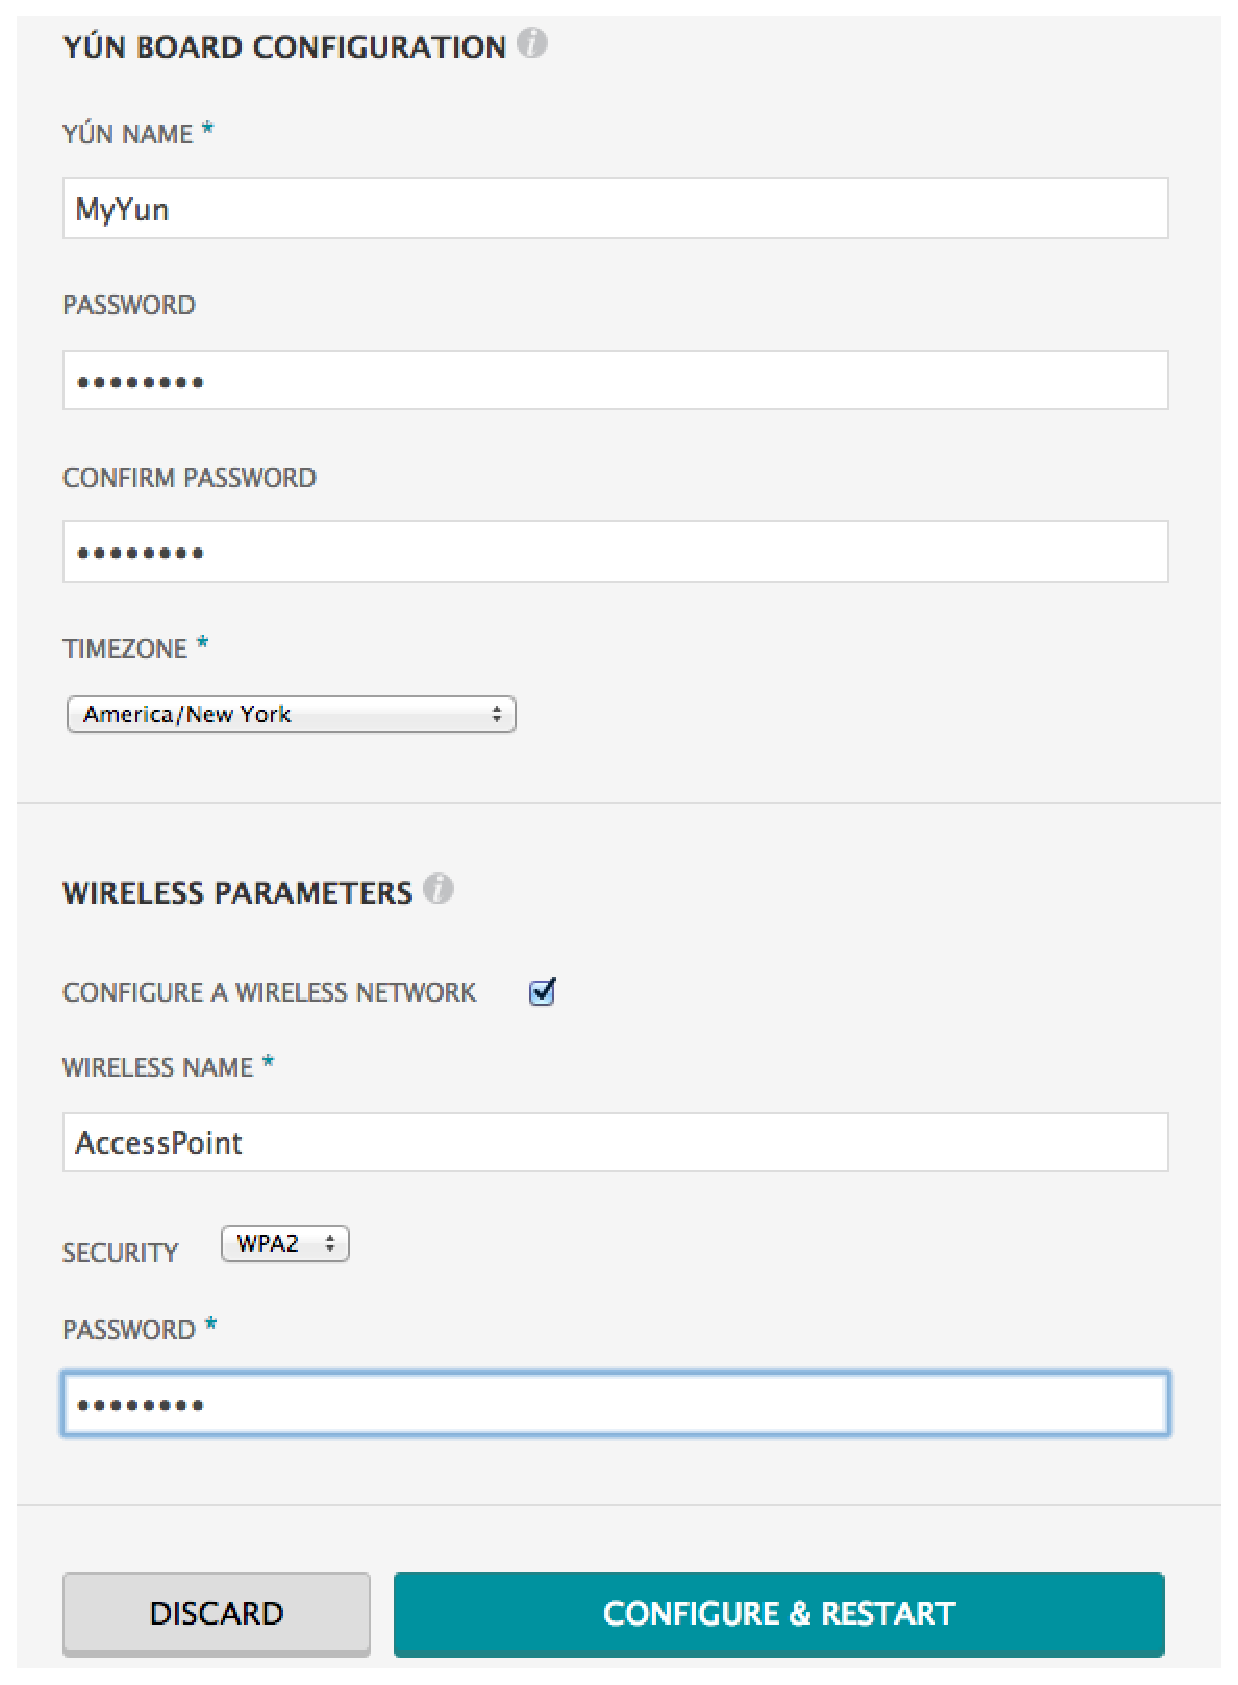
\includegraphics[keepaspectratio,width=0.6\textwidth]{YunWebConfig.eps}
    \caption{Arduino Yún Web Config}\label{fig:yun-web-config}
\end{figure}

Una vez se guarda la nueva configuración la distribución Linux se reinicia y automáticamente se conectará a la red WiFi que hayamos establecido, indicándonos que nos conectemos a la misma WiFi mediante la siguiente ventana:

\begin{figure}[H]
    \centering
    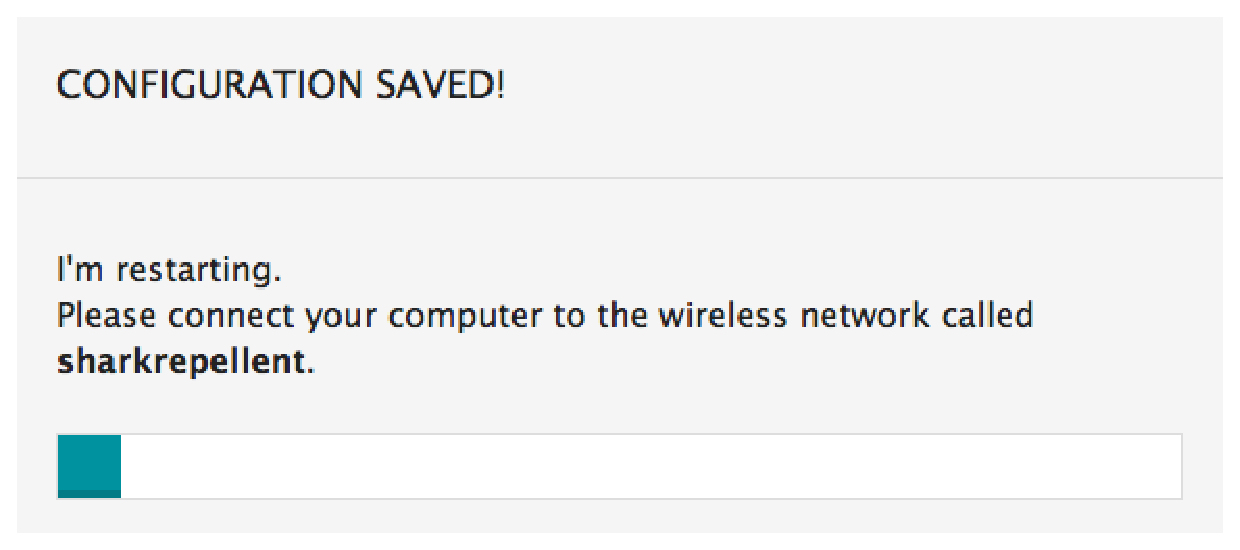
\includegraphics[keepaspectratio,width=0.6\textwidth]{YunRebooting.eps}
    \caption{Arduino Yún Web Rebooting}\label{fig:yun-web-rebooting}
\end{figure}

Pasado varios segundos automáticamente se nos volverá a conectar a la página de configuración de Arduino donde tendremos que introducir la nueva contraseña para acceder.

\subsection{Problemas detectados}

La versión de Linux que trae la placa Arduino no viene con las librerías para utilizar el puerto USB en modo HID (\emph{Human Interface Device}) por lo que no reconoce el lector de códigos de barras USB. Para configurarlo se han tenido que bajar las librerías e instalarlas a través de SSH.

\begin{enumerate}

	\item Descargar y guardar en la memoria micro-sd (\emph{/mnt/sda1/}) las dos siguientes librerías:

		\begin{itemize}
			\item kmod-hid-generic\_3.8.3-1\_ar71xx.ipk
			\item kmod-hid\_3.8.3-1\_ar71xx.ipk
		\end{itemize}

	\item Actualizar el sistema de paquetes e instalar las dos siguientes librerías para permitir la instalación de las librerías anteriores:

		\begin{lstlisting}
opkg update
opkg install kmod-input-core
opkg install kmod-input-evdev
		\end{lstlisting}

	\item Instalar las librerías de la micro-sd:

		\begin{lstlisting}
rm /tmp/opkg-lists/*
opkg install /mnt/sda1/kmod-hid\_3.8.3-1\_ar71xx.ipk
opkg install /mnt/sda1/kmod-hid-generic\_3.8.3-1\_ar71xx.ipk
		\end{lstlisting}

	\item Instalar el driver HID:

		\begin{lstlisting}
opkg update
opkg install kmod-usb-hid
		\end{lstlisting}

	\item Cargar el driver HID en el Kernel:

		\begin{lstlisting}
insmod hid-generic
echo "hid-generic" >>/etc/modules.d/62-hid-generic
		\end{lstlisting}

	\item Reiniciar Linux:

		\begin{lstlisting}
reboot
		\end{lstlisting}

	\item Enchufar el lector de tarjetas USB y comprobar que funciona:

		\begin{lstlisting}
cat /dev/input/event1 | hexdump
		\end{lstlisting}

\end{enumerate}

Con esta configuración Linux es capaz de cargar el dispositivo USB, pero, si se desenchufa y se vuelve a enchufar a veces no carga y da problemas. Por suerte, el \emph{23 de Abril de 2014} han sacado una nueva versión de \emph{OpenWrt-Yun} que corrige estos errores, e introduce las siguientes mejoras:

	\begin{itemize}
		\item OpenWrt
			\begin{itemize}
 				\item wget now supports ssl
 				\item Fixed fuses values in run-avrdude
 				\item nano is now built-in (no need to become ''vi'' experts any more)
 				\item Updated ruby to 1.9.3-p429
 				\item Fixed USB port stability (when using it both with a pen drive or as a serial device)
 				\item Patched dhcp script to fix ethernet routing issue
 				\item Added lots of webcam modules
 				\item Fixed USB keyboard support
 				\item Heartbleed http://heartbleed.com/
 				\item Linux side ready visual notification: when linux boot completes, the usb led lights up (it's bright white)
 				\item Disk space expander tutorial: using an micro SD card to have gigabytes of disk space
 				\item Added ''upgrade-all'' script for easier massive upgrade of packages (available only after having followed the ExpandingYunDiskSpace tutorial)
 				\item Node.js is now available as an optional package: other native nodejs packages include bleno, noble, serialport, socket.io.
			\end{itemize}

		\item Web panel
			\begin{itemize}
				\item Previously, jsonp calls were triggered by the ''jsonp'' query string parameter only. Now, you can use ''callback'' as well.
				\item Added Mailbox support
				\item Various fixes
			\end{itemize}

		\item Bridge
			\begin{itemize}
				\item File.size() now implemented
				\item PHP bridge client (thx Luca Saltoggio)
				\item Bridge is now run with ''-u'' python flag, preventing some random lockups in the Bridge
				\item Resolved conflict with python ''json'' module
			\end{itemize}
	\end{itemize}

Una vez actualizado la versión de \emph{OpenWrt-Yun} siguiendo las instrucciones de la página de Arduino (\emph{http://arduino.cc/en/Tutorial/YunSysupgrade}) solamente tenemos que instalar la librería USB HID por SSH (ya que sigue sin venir por defecto):

	\begin{lstlisting}
opkg update
opkg install kmod-usb-hid
	\end{lstlisting}

Y nos funcionará el lector de códigos de barras USB sin ningún problema, aunque se desenchufe y se vuelva a enchufar.

\subsection{Decodificando el lector de código de barras}

El siguiente problema a resolver es la creación de un script en python que permita la lectura de códigos de barras. Para ello se ha tenido que decodificar los caracteres que envía al sistema operativo, y una vez hecho, comprender como funciona.

El funcionamiento es muy sencillo. Cuando el lector de código de barras encuentra un código válido lo envía al sistema por letras y por último, y es lo que nos ayuda a comprender que ha terminado de enviarnos el código de barras, nos envía dos caracteres seguidos (\emph{Control + j}) que simbolizan el salto de línea (\emph{Line Feed}).

El siguiente script nos permite leer los caractéres escaneados e imprimirlos por consola o enviarlos al microcontrolador a través de la librería \emph{Bridge}.

\begin{lstlisting}
#!/usr/bin/python
# -*- coding: utf-8 -*-

import struct
import time
import sys
sys.path.insert(0, '/usr/lib/python2.7/bridge/')

from bridgeclient import BridgeClient as bridgeclient

# Variables
infile_path = "/dev/input/event1"

#long int, long int, unsigned short, unsigned short, unsigned int
FORMAT = 'llHHI'
EVENT_SIZE = struct.calcsize(FORMAT)

teclasPulsadas = dict()
escribiendoLetras = False
codigoBarras = ''
bridgeCliente = bridgeclient()
in_file = None

# Funciones

def esTeclaNumerica(value):
    return value >= 458782 and value <= 458791

def getNumero(value):
    return (value - 458781)%10

def esTeclaLetra(value):
    return (value >= 458756 and value <= 458781)

def getLetra(value):
    posicionValue = value - 458756
    asciiValue = posicionValue + 65
    return str(unichr(asciiValue))

# 458792 -> Intro
# 458976 + 458765 (Control + j => Line Feed)
def esTeclaControl(value):
    return value == 458792 or \
            value == 458976 or \
            value == 458765
def procesarEvento(event):
    global teclasPulsadas, escribiendoLetras, codigoBarras, bridgeCliente
    (tv_sec, tv_usec, type, code, value) = struct.unpack(FORMAT, event)

    # Importa este orden de la condicion, si se altera puede imprimir
    # caracteres escritos muy deprisa en otro orden
    if value not in teclasPulsadas:
        teclasPulsadas[value] = 'S'
    else:
        if esTeclaControl(value) and escribiendoLetras:
            escribiendoLetras = False
            print codigoBarras
            #bridgeCliente.put('codebar', codigoBarras)

            codigoBarras = ''
        elif not esTeclaControl(value) and \
                (esTeclaNumerica(value) or \
                esTeclaLetra(value)):
            escribiendoLetras = True
            if esTeclaNumerica(value):
                codigoBarras += str(getNumero(value))
            elif esTeclaLetra(value):
                codigoBarras += getTeclaLetra(value)
        del teclasPulsadas[value]

def conectarUsb():
    global in_file
    in_file = None
    conectado = False
    while not conectado:
        try:
            # Intentamos abrir el fichero
            in_file = open(infile_path, "rb")
            conectado = True
        except IOError:
            time.sleep(1) # Pausamos 1seg

# Inicio programa
conectarUsb()
event = in_file.read(EVENT_SIZE)
while event:
    try:
        procesarEvento(event)
        event = in_file.read(EVENT_SIZE)
    except IOError:
        conectarUsb()
        event = in_file.read(EVENT_SIZE)
\end{lstlisting}

\chapter{CONCLUSIONES}

Este proyecto ha abordado el diseño y la construcción de un componente hardware apoyado por una plataforma en la nube para el seguimiento del consumo en el hogar, en concreto las compras realizadas en los supermercados. Para ello, se ha utilizado \emph{Arduino Yún} y una serie de componentes en el diseño del prototipo y de distintas tecnologías web para la construcción de la aplicación web.

La elección de este proyecto surgió de la curiosidad acerca de \emph{Arduino}, del creciente entusiasmo en cuantificar todo lo que se pueda y de la multitud de aplicaciones que se utilizan para llevar el control de los gastos en el hogar.

\section{Primer paso}

El primer paso en el proyecto fue hacerse con un \emph{Arduino} para empezar a jugar con él y familiarizarse con su entorno de programación. Simultáneamente se adquirió un lector de código de barras con conector \emph{USB HID}.

La versión de \emph{Arduino} elegida fue la \emph{UNO} debido a que su precio económico y a la amplia documentación que hay sobre la placa. El primer problema que se tuvo fue la falta de conexión \emph{USB} de la placa, se resolvió adquiriendo una \emph{Shield USB}. El segundo problema vino por la falta de conexión \emph{WiFi}, se intentó resolver adquiriendo una \emph{Shield WiFi} no oficial, pero no se logró hacer que funcionara.

Con estos problemas el segundo paso consistió en investigar y en conocer \emph{Arduino Yún}, una placa \emph{Arduino} que resuelve estos problemas ya que dispone de un puerto \emph{USB} y de un microprocesador con \emph{Linux} y conexión \emph{WiFi}. Con todos los componentes adecuados se diseñó el primer software para el escaneo de códigos de barras, el cual se guardaba a través de \emph{Internet} en un servidor.

\section{Segundo paso}

El segundo paso consistió en desarrollar la aplicación servidor utilizando para ello algunas de las piezas que componen las metodologías ágiles; control de versiones, tests unitarios e integración contínua.

\begin{itemize}

    \item Para el control de versiones se ha utilizado \emph{GitHub}, una plataforma que permite la creación de repositorios públicos de manera gratuita y que actualmente es la que más auge tiene en los proyectos de código abierto.

    \item Para los tests unitarios se ha utilizado \emph{PHPUnit} debido a que es uno de los frameworks más conocidos. Se tuvieron que resolver problemas con \emph{CodeIgniter} ya que no está pensado para realizar tests sobre él.

    \item Para la integración contínua se ha utilizado \emph{TravisCI}, una herramienta web que se sincroniza con tu cuenta de \emph{GitHub} para construir y pasar los tests unitarios de todas las modificaciones que realices sobre el repositorio.

\end{itemize}

\section{Tercer paso}

A continuación, con las primeras versiones de la aplicación servidor, se fue realizando el diseño de la página web utilizando para ello \emph{Bootstrap} y algunas librerías \emph{JavaScript} como; \emph{JQuery}, \emph{Director}, \emph{Handlebars}, etc.

\section{Cuarto paso}




\chapter{LÍNEAS FUTURAS}

La principal motivación de este proyecto es acercar la tecnología a una de las actividades cotidianas que menos ha cambiado a lo largo de la historia; realizar la compra.

Para ello se ha diseñado un dispositivo que permita cuantificar y ofrecer información al usuario acerca de sus compras. Por ejemplo, permitir consultar los productos que dispone en el frigorífico, las compras que ha realizado a lo largo del tiempo, análisis de gastos, etc.

Las grandes compañías a nivel mundial aún no han dado el salto a utilizar este tipo de tecnologías en sus productos convencionales. Sí disponen de algún frigorífico de gama alta con tecnología futurista, los cuales, no son accesibles para el consumidor medio.

Por ello, con este proyecto se pretende acercar al consumidor a parte de esta tecnología futurista. A través de un componente sencillo, barato y elegante. Así, con el objetivo de poder comercializar realmente este proyecto se proponen las siguientes líneas futuras.

\section{COMPONENTE HARDWARE}

El componente hardware que se ha diseñado es un prototipo funcional del producto final. Pero, para una comercialización del producto es recomendable realizar las siguientes innovaciones:

\begin{itemize}
    \item Miniaturización

        El componente que más ocupa del prototipo es el lector de código de barras. Es necesario encontrar un proveedor que proporcione un lector pequeño y discreto, de esta manera se puede integrar en la parte inferior del producto sin ocupar un gran espacio.

    \item Diseño

        Fribone es un producto pensado para el hogar, en concreto, la cocina. Por lo que tiene que ser un producto elegante e integrador, nadie quiere un producto que rompa la armonía de la cocina.

    \item Ergonomía

        La mayoría de las personas experimentan algún grado de limitación física en algún momento de su vida. Por lo tanto, el diseño final del producto, además de ser elegante, debe estar pensado para que pueda ser manejado por personas con ciertas discapacidades físicas.

        Una manera de afrontar esta tarea es pensar en la eliminación de los botones del aparato, que pueden ser difíciles de pulsar, y añadir una pantalla más grande y con respuesta táctil. Así, se puede realizar una interfaz con unos botones en pantalla grandes y visibles.

\end{itemize}

\section{COMPONENTE SERVIDOR Y SOFTWARE}

La arquitectura y diseño del software ha seguido una metodología ágil. Así, se ha conseguido levantar una infraestructura usable en un tiempo breve. Gracias a los tests unitarios y a la plataforma de integración continua, \emph{TravisCI}, se pueden seguir desarrollando pequeños cambios incrementales para dotar de más potencia a la aplicación:

\begin{itemize}

    \item Universalidad

        Integrar soluciones de acceso a la plataforma a partir de otros servicios (\emph{Facebook}, \emph{Google}, etc.), y ofrecer una \emph{API RESTful} basada en \emph{OAuth 2} para la autorización del acceso a la información.

    \item Data Mining

        Explorar y buscar nuevas técnicas de análisis de la información que ingresan los usuarios para poder ofrecerles sugerencias en base a sus gustos, consejos a la hora de comprar, etc.

    \item Servicios a terceros

        Animar a las compañías del sector comercial a ofrecer sus productos a través de la plataforma. De esta manera, se le pueden ofrecer nuevas experiencias al usuario como la planificación de compras automáticas en base a los productos que dispone en su frigorífico.
    \end{itemize}

%%%%%%%%%%%%%%%%%%%%%%%%%%%%%%%%%%%%%%%%%%%%%%%%%%%%%%%%%%%%%%%
% Bibliografía
%%%%%%%%%%%%%%%%%%%%%%%%%%%%%%%%%%%%%%%%%%%%%%%%%%%%%%%%%%%%%%%



\nocite{*}
\bibliographystyle{plain}
\bibliography{bibliografia/fribone-bibliografia}{}

\end{document}